\documentclass{paper}
\usepackage{nomencl}
\usepackage{amsmath}
\usepackage{graphicx}
\usepackage{subfigure}
\usepackage{parskip}
\usepackage[toc,page]{appendix}
\usepackage{csquotes}
\usepackage{framed}
\usepackage{amsthm}

\theoremstyle{definition}
\newtheorem{exmp}{Example}[section]

\theoremstyle{theorem}
\newtheorem{theorem}{Theorem}[section]
 
\theoremstyle{definition}
\newtheorem{definition}{Definition}[section]

\theoremstyle{remark}
\newtheorem{remark}{Remark}[section]

\title{Hardware for Self-driving Cars}
\author{A. Giavaras}
\date{}

\begin{document}
\maketitle
\tableofcontents

\clearpage
\section{Hardware for Self-driving Cars}
\label{hardware_for_self_driving_cars}

In this chapter, we will discuss sensors, and the various types of them
available for the task of perception. Next we will discuss the self-driving car hardware available nowadays. 

\subsection{Sensors}
\label{sensors}

Let's begin by talking about sensors. Even the best perception algorithms
are limited by the quality of their sensor data. And careful selection of sensors
can go a long way to simplifying the self-driving perception task. Let's try to give a definition of
what a sensor is.


\begin{framed}
\theoremstyle{definition}
\begin{definition}{\textbf{What is a sensor? }}

For our purposes, a sensor is any device that measures or
detects some property of the environment, or changes to that property over time.
\end{definition}
\end{framed}

Sensors are broadly categorized into two types, depending on what property they record. If they record a property of
the environment they are called {\textbf{exteroceptive}}. Extero means outside, or from the surroundings. On the other hand, if the sensors
record a property of the ego vehicle, they are called {\textbf{proprioceptive}}. Proprios means internal, or one's own. Let's start by discussing
common exteroceptive sensors. 

\subsubsection{Camera}

We start with the most common and widely used sensor in autonomous driving, the camera. Cameras are a passive, light-collecting
sensor that are great at capturing rich, detailed information about a scene. In fact, some groups believe that the
camera is the only sensor truly required for self-driving. But state of the art performance is
not yet possible with vision alone. While talking about cameras, we usually tend to talk about three
important comparison metrics. We select cameras in terms:


\begin{itemize}
\item resolution
\item field of view or FOV
\item dynamic range
\end{itemize}

The resolution is the number of pixels that create the image. So it's a way of specifying
the quality of the image.  The field of view is defined by the horizontal and vertical angular extent that is visible to the camera, and can be
varied through lens selection and zoom. The dynamic range of the camera is the difference between the darkest and the lightest tones in an image. High dynamic range is critical for
self-driving vehicles due to the highly variable lighting conditions encountered
while driving especially at night. 

There is an important trade off cameras and lens selection, that lies between the choice of
field of view and resolution. Wider FOV permits a lager
viewing region in the environment, but fewer pixels that absorb light from one particular object. As the FOV increases, we need to increase resolution to still be
able to perceive with the same quality, the various kinds of information we may encounter. 
Other properties of cameras that affect perception exist as well, such as focal length, depth of field and frame rate. 
 
The combination of two cameras with overlapping fields of view and aligned image planes is
called the stereo camera. Stereo cameras allow depth estimation
from synchronized image pairs. Pixel values from image can be
matched to the other image producing a disparity map of the scene. This disparity can then be used
to estimate depth at each pixel. 

\subsubsection{LIDAR}

Next we have LIDAR which stands for light detection and ranging sensor. LIDAR sensing involves shooting
light beams into the environment and measuring the reflected return. By measuring the amount of returned
light and time of flight of the beam. Both in intensity in range to
the reflecting object can be estimated. An illustration of LIDAR based environment representation is shown in figure \ref{lidar_illustrate}.

\begin{figure}[!htb]
\begin{center}
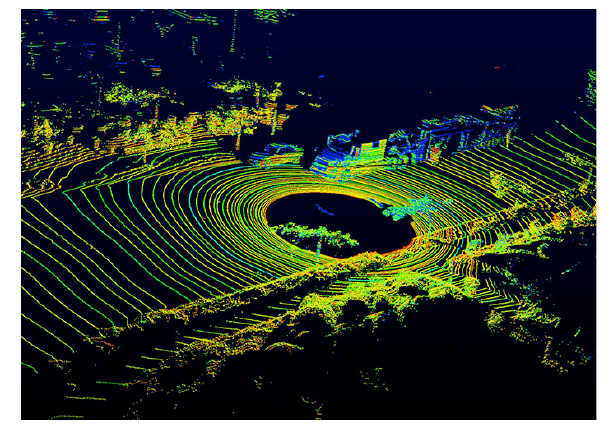
\includegraphics[scale=0.280]{img/hardware/lidar_illustrate.jpeg}
\end{center}
\caption{LIDAR illustration of environment representation.}
\label{lidar_illustrate}
\end{figure}

LIDAR usually includes a spinning element
with multiple stacked light sources and outputs a three dimensional
point cloud map, which is great for assessing scene geometry. Because it is an active sensor
with it's own light sources, LIDAR are not effected by
the environments lighting. So LIDAR do not face the same challenges
as cameras when operating in poor or variable lighting conditions. Let's discuss the important comparison
metrics for selecting LIDAR.

\begin{itemize}
\item The first is the number of sources it contains with 8, 16, 32, and 64 being common sizes. 
\item the second is the points per second it can collect. The faster the point collection, the more
detailed the 3D point cloud can be. 
\end{itemize}

Another characteristic is the rotation rate. The higher this rate, the faster
the 3D point clouds are updated. Detection range is also important, and is dictated by the power
output of the light source. And finally, we have the field of view,
which once again, is the angular extent
visible to the LIDAR sensor. 

Finally, we should also mention the new
LIDAR types that are currently emerging. High-resolution, solid-state LIDAR. Without a rotational component
of the typical LIDARs, these sensors stand to become
extremely low-cost and reliable. Thanks to being implemented
entirely in silicon. HD solid-state LIDAR
are still a work in progress. But definitely something exciting for
the future of affordable self-driving. 

\subsubsection{Radar}

Our next sensor is RADAR, which stands for radio detection and ranging. RADAR sensors have been
around longer than LIDAR and robustly detect large objects in the environment. They are particularly useful in adverse
weather as they are mostly unaffected by precipitation. Let's discuss some of the comparison
metrics for selecting RADAR. RADAR are selected based on

\begin{itemize}
\item detection range
\item field of view, 
\item the position and speed measurement accuracy. 
\end{itemize}

RADARs are also typically available as either having a wide angular field of view but short range. 
Or having a narrow FOV but a longer range. 


\subsubsection{Ultrasonics or sonars}

The next sensor we are going to discuss are ultrasonics or sonars. Originally so named for
sound navigation and ranging. Which measure range using sound waves. Sonars are sensors that are short
range and inexpensive ranging devices. This makes them good for parking scenarios, where the ego-vehicle needs to make
movements very close to other cars. Another great thing about sonar is that they are low-cost. Moreover, just like RADAR and LIDAR,
they are unaffected by lighting and precipitation conditions. A sonar sensor is selected based
on a few key metrics itemized next. 

\begin{itemize}
\item The maximum range they can measure
\item The the detection FOV
\item The cost
\end{itemize}

\subsubsection{Proprioceptive sensors}

Now let's discuss the proprioceptive sensors, the sensors that sense ego properties. The most common ones here
are:

\begin{itemize}
\item Global Navigation Satellite Systems, GNSS for short, such as GPS or Galileo
\item Inertial Measurement Units or IMU's
\item Wheel odometers
\end{itemize}

GNSS receivers are used to measure ego vehicle position, velocity, and sometimes heading. The accuracy depends a lot on
the actual positioning methods and the corrections used. Apart from these, the IMU also
measures the angular rotation rate, accelerations of the ego vehicle, and
the combined measurements can be used to estimate the 3D orientation
of the vehicle. Where heading is the most important for
vehicle control. Finally, we have wheel odometry sensors. This sensor tracks the wheel
rates of rotation, and uses these to estimate the speed and
heading rate of change of the ego car. This is the same sensor that tracks
the mileage on your vehicle. 

In summary, the major sensors used nowadays for autonomous driving perception
include cameras, RADAR, LIDAR, sonar, GNSS, IMUs,
and wheel odometry modules. These sensors have many characteristics that can vary wildly, including resolution,
detection range, and FOV. 

Selecting an appropriate sensor configuration for a self-driving car is not trivial. Figure \ref{sensors_positioning} is a simple graphic that
shows each of the sensors and where they usually go on a car. 

\begin{figure}[!htb]
\begin{center}
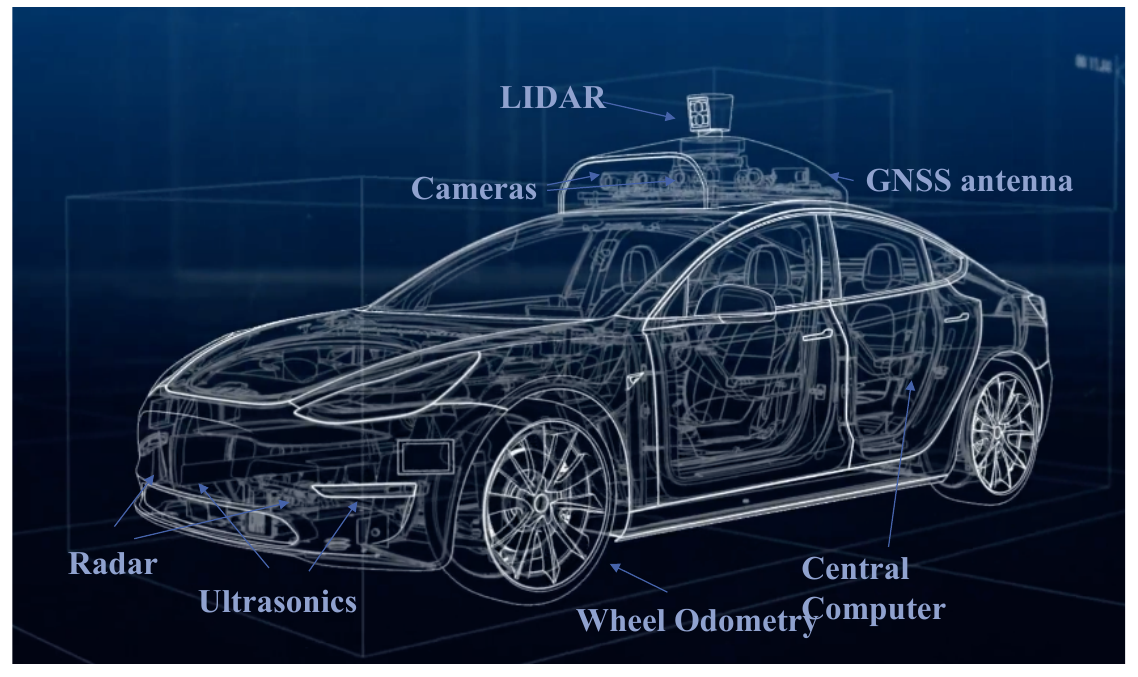
\includegraphics[scale=0.280]{img/hardware/sensors_positioning.jpeg}
\end{center}
\caption{Usual sensor positioning.}
\label{sensors_positioning}
\end{figure}


\subsection{Computing Hardware}
\label{computing_hardware}

Let's now discuss a little bit about the computing hardware most commonly used in  self-driving cars at the time of writing. The most crucial part
is the computing brain, the main decision making unit of the car. It takes in all sensor data and outputs
the commands needed to drive the vehicle. Most companies prefer to design their own
computing systems that match the specific requirements of their sensors and
algorithms. Some hardware options exist, however, that can handle self-driving computing loads out of the box. 

The most common examples would be Nvidia's Drive PX and Intel \& Mobileye's EyeQ. Any computing brain for self-driving needs
both serial and parallel compute modules. Particularly for image and LIDAR processing to do segmentation, object detection, and mapping. 
For these we employ GPUs, FPGAs and custom ASICs (Application Specific Integrated Circuit), which are specialized hardware to
do a specific type of computation. 

For example, the drive PX units include multiple GPUs. The EyeQs have FPGAs both to
accelerate parallalizable compute tasks, such as image processing or
neural network inference. 

Finally, a quick comment about synchronization. Because we want to make driving
decisions based on a coherent picture of the road scene. It is essential to correctly synchronize
the different modules in the system, and serve a common clock. Fortunately, GPS relies on extremely
accurate timing to function, and as such can act as an appropriate
reference clock when available. Regardless, sensor measurements must be
timestamped with consistent times for sensor fusion to function correctly. Let's summarize. In this video,
we learned about sensors and their different types based
on what they measure. 

\subsection{Hardware Configuration}
\label{hardware_configuration}

Section \ref{sensors}, covers the various kinds of sensors most commonly used for perception. 
One question that should be answered is how do we place these sensors on the vehicle in order to  aquire a complete view of the environment? 


In this section, we will discuss the configuration design to meet sensor coverage needs for an autonomous driving car. 
We will do this by going through two common scenarios:

\begin{itemize}
\item Driving on a highway and 
\item Driving in an urban environment
\end{itemize}
 
After analyzing these scenarios, we will lay out the overall coverage requirements and discuss some issues with the design. 

Let's however begin by recalling the most commonly available sensors. These are:

\begin{itemize}
\item The camera for appearance input. 
\item The stereo camera for depth information
\item Lidar for all whether 3D input
\item Radar for object detection
\item Ultrasonic for short-range 3D input 
\item GNSS/IMU data and wheel odometry for ego state estimation. 
\end{itemize}

Also, remember that all of these sensors come in different configurations and  different ranges in FOV over which they can sense. 
They have some resolution that depends on the instrument specifics and the field of view. Before we move to discussing coverage, let's define the deceleration rates we're willing to accept for driving which will drive the detection ranges needed for our sensors. 


\begin{framed}
\theoremstyle{remark}
\begin{remark}{\textbf{Aggressive Deceleration}}

Aggressive deceleration is set to $5 m/sec^2$ which is roughly the deceleration you experience when you slam the brakes hard and try to stop abruptly in case of an emergency. 
\end{remark}
\end{framed}

Normal decelerations are set to $2 m/sec^2$, which is reasonably comfortable while still allowing the car to come to a stop quickly. 
Given a constant deceleration our braking distance $d$ can be computed as follows according to equation \ref{stopping_distance}.

\begin{equation}
d = \frac{V^2}{2\alpha}
\label{stopping_distance}
\end{equation}

where $V$ is the vehicle velocity and  $\alpha$ is its rate of deceleration. 
We can also factor in reaction time of the system and road surface friction limits, but we'll keep things simple in this discussion. 

Let's talk about coverage now. The question we want to answer is where should we place our sensors so that we have sufficient input for our driving task? 
Practically speaking, we want our sensors to capture the ODD we have in mind or the ODD our system can produce decisions for. 
We should be able to provide all of the decisions with sufficient input. 
There can be so many possible scenarios in driving but we'll look at just two common scenarios to see how the requirements drive our sensor selection. 
Will look at highway and urban driving. Let's think about these two situations briefly. 


For a divided highway, we have fast moving traffic, usually high volume, and quite a few lanes to monitor, 
but all vehicles are moving in the same direction. The other highlight of driving on a highway setting is that there are 
fewer and gradual curves and we have exits and merges to consider as well. 

On the other hand, in the urban situation we'll consider, 
we have moderate volume and moderate speed traffic with fewer lanes but with 
traffic moving in all directions especially through intersections. 

\subsubsection{Highway Scenario}

Let's start with the highway setting. 
We can break down the highway setting into three basic maneuver needs. 

\begin{itemize}
\item We may need to hit the brakes hard if there's an emergency situation. 
\item We need to maintain a steady speed matching the flow of traffic around us.
\item We might need to change lanes. 
\end{itemize}

In the case of an emergency stop, if there is a blockage on our road we want to stop in time. 
So, applying our stopping distance equation longitudinally, we need to be able to sense about a 110 meters in front of us assuming a highway speed of a 120 kilometers and aggressive deceleration. 
Most self-driving systems aim for sensing ranges of a 150 to 200 meters in front of the vehicle as a result. 
Similarly, to avoid lateral collision or to change lanes to avoid hitting an obstacle in our lane, we need to be able to sense at least our adjacent lanes, 
which are 3.7 meters wide in North America. To maintain speed during vehicle following, we need to sense the vehicle in our own lane. 
Both their relative position and the speed are important to maintain a safe following distance. 
This is usually defined in units of time for human drivers and set to two seconds in nominal conditions. 
It can also be assessed using aggressive deceleration of the lead vehicle and the reaction time from our ego vehicle. 
So, at a 120 kilometers per hour, relative position and speed measurements to a range of 165 meters are needed and typical systems use 100 meters for this requirement. 
Laterally, we need to know what's happening anywhere in our adjacent lanes in case another vehicles seeks to merge into our lane or we need to merge with other traffic. 
A wide 160 to 180 degree field of view is required to track adjacent lanes and a range of 40 to 60 meters is needed to find space between vehicles. 

Finally, let's discuss the lane change maneuver and consider the following scenario. 
Suppose we want to move to the adjacent lane, longitudinally we need to look forward, so we are a safe distance from the leading vehicle and 
we also need to look behind just to see what the rear vehicles are doing and laterally it's a bit more complicated. 
We may need to look beyond just the adjacent lanes. For example, what if a vehicle attempts to maneuver into the adjacent lane at the same time as we do? 
We'll need to coordinate our lane change room maneuvers so we don't crash. 

The sensor requirements for lane changes are roughly equivalent to those in the maintain speed scenario. 
As both need to manage vehicles in front of and behind the ego vehicle as well as to each side. 
Overall, this gives us the picture for coverage requirements for the highway driving scenario. 
We need longitudinal sensors and lateral sensors and both wide and narrow FOV sensors to do these three maneuvers, the emergency stop, maintaining speed and changing lanes. 
Already from this small set of ODD requirements we see a large variety of sensor requirements that arise. 


\begin{figure}[!htb]
\begin{center}
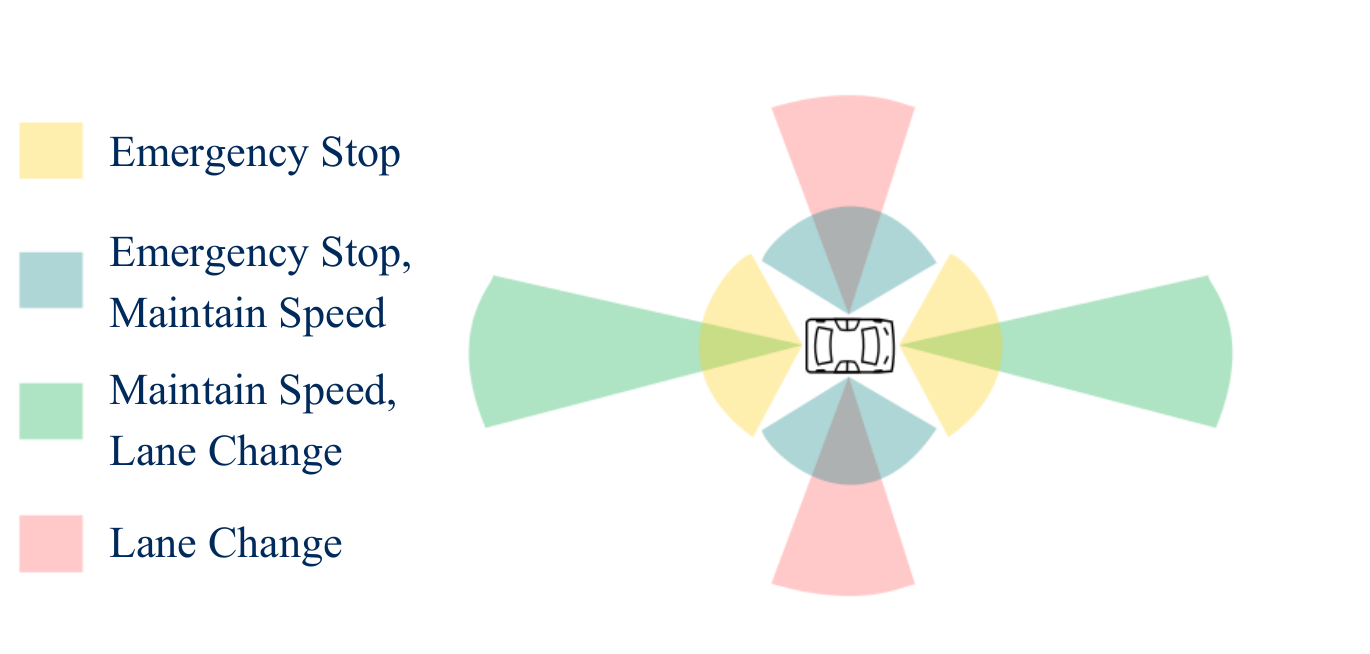
\includegraphics[scale=0.280]{img/hardware/highway_analysis_overall_coverage.jpeg}
\end{center}
\caption{Highway analysis overall coverage.}
\label{highway_analysis_overall_coverage}
\end{figure}

\subsubsection{Urban Scenario}
\label{urban_scenario}

Let's discuss the urban scenario next. 
The urban scenario as we discussed before is a moderate volume, moderate traffic scenario with fewer lanes on the highway case but with the added complexity of pedestrians. 
There are six types of basic maneuvers here. Obviously, we can still perform emergency stop, maintain speed and lane changes but we also have scenarios such as overtaking a parked car, 
left and right turns at intersections and more complex maneuvers through intersections such as roundabouts. 
In fact, for the first three basic maneuvers, the coverage analysis is pretty much the same as the highway analysis but since we are not moving as quickly, 
we don't need the same extent for our long-range sensing. 

Let's discuss the overtake maneuver next. 
More specifically, consider a case where you have to overtake a parked car. 
Longitudinally, we definitely need to sense the parked car as well as look for oncoming traffic. 
So, we need both sensors, wide short-range sensors to detect the parked car and narrow long-range sensors to identify if oncoming traffic is approaching. 
Laterally, we'll need to observe beyond the adjacent lanes for merging vehicles as we did in the highway case. 
Intersections require that  we  have near omni-directional sensing for all kinds of movements that can occur. 
Approaching vehicles, nearby pedestrians, doing turns and much more. 
Finally, for roundabouts we need a wide-range, short distance sensor laterally since the traffic is slow but 
we also need a wide-range short distance sensor longitudinally because of how movement around the roundabout occurs. 
We need to sense all of the incoming traffic flowing through the roundabout to make proper decisions. 

Thus, we end up with the overall coverage diagram for the urban case shown in figure \ref{urban_analysis_overall_coverage}. 
The main difference with respect to highway coverage is because of the sensing we require 
for movement at intersections and at roundabouts and for the overtaking maneuver. 
In fact, the highway case is almost entirely covered by the urban requirements. 


\begin{figure}[!htb]
\begin{center}
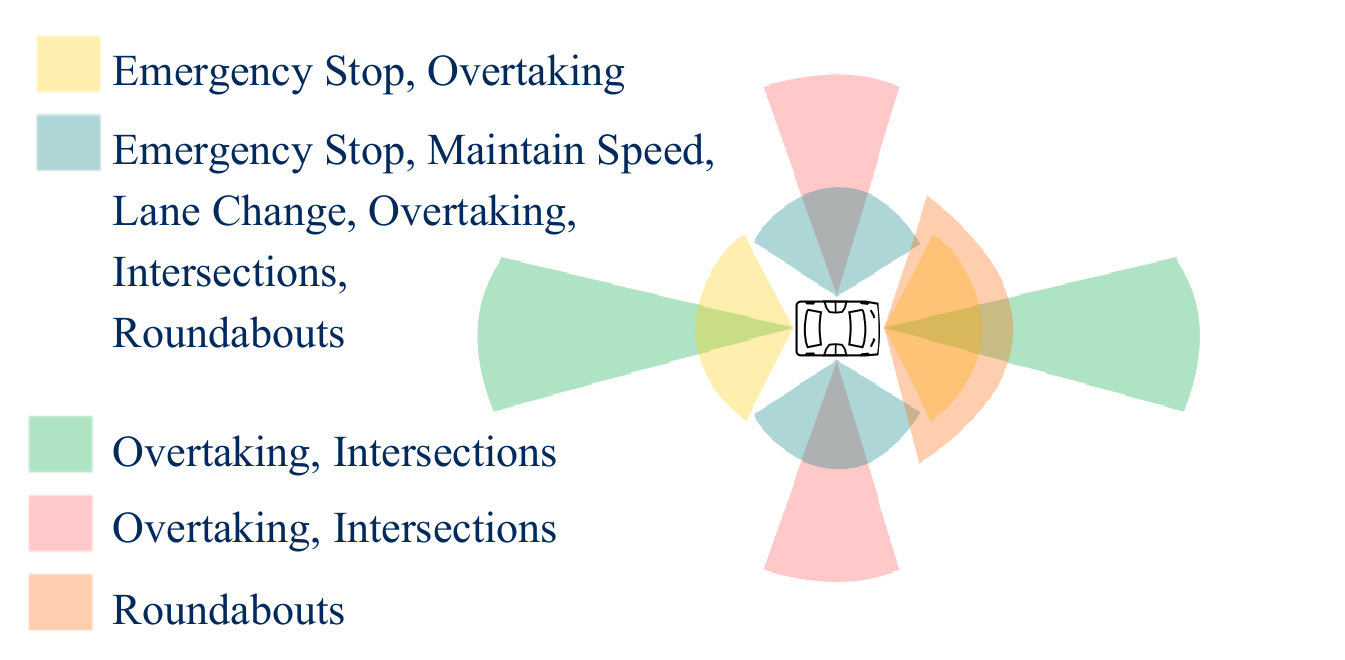
\includegraphics[scale=0.280]{img/hardware/urban_analysis_overall_coverage.jpeg}
\end{center}
\caption{Urban analysis overall coverage.}
\label{urban_analysis_overall_coverage}
\end{figure}


Let's summarize the coverage analysis. For all of the maneuvers we do, we need long range sensors which typically 
have shorter angular field of view and wide angular field of view sensors which typically have medium to short-range sensing. 
As the scenarios become more complex, we saw the need for full 360 degrees sensor coverage on the short scale out to 
about 50 meters and much longer range requirements in the longitudinal direction. 
We can also add even shorter range sensors like sonar which are useful in parking scenarios and so in the end our sensor configuration looks something like this diagram. 


\begin{figure}[!htb]
\begin{center}
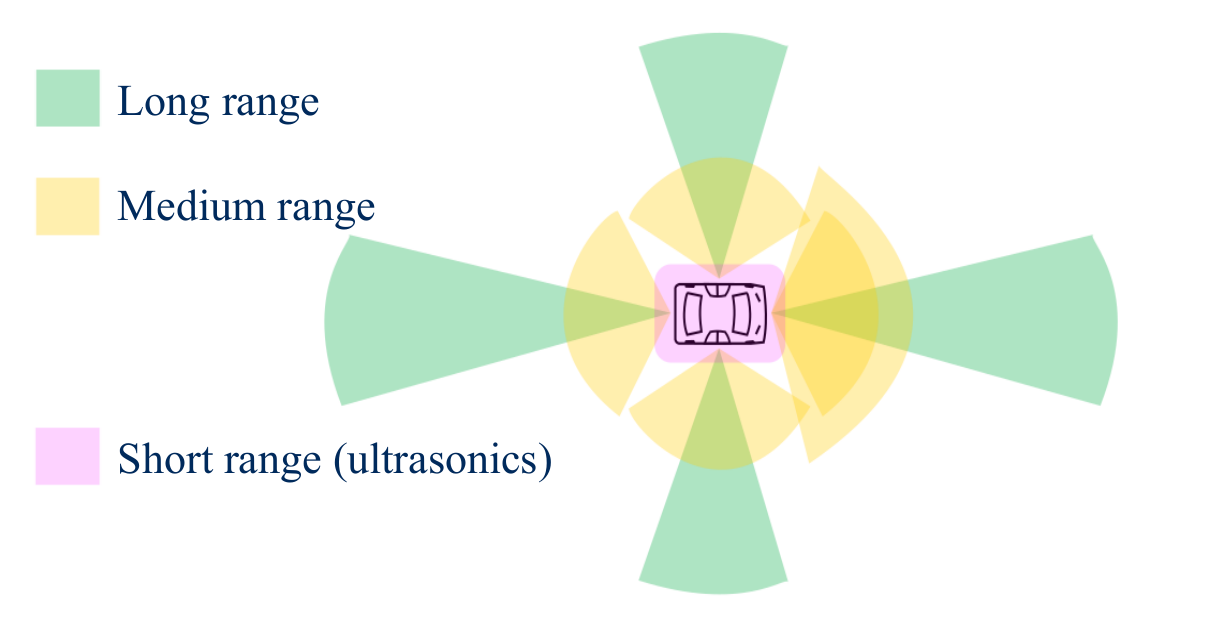
\includegraphics[scale=0.280]{img/hardware/overall_coverage.jpeg}
\end{center}
\caption{Overall coverage.}
\label{overall_coverage}
\end{figure}


To summarize, our choice of sensors should be driven by the requirements of the maneuvers we want to execute and it should include 
both long-range sensors for longitudinal dangers and wide field of view sensors for omnidirectional perception. 
The final choice of configurations also depends on our requirements for operating conditions, sensor redundancy due to failures and on budget. 
There is no single answer to which sensors are needed for a self-driving car. 



\section{Sensor Calibration}
\label{sensor_calibration}

Now that we've seen how we can combine multiple sources
of sensor data to estimate the vehicle state, it's time to address the topic of \textbf{sensor calibration}.
Sensor calibration and is absolutely essential for doing state estimation properly. Concretely, in this section,
we will discuss the three main types of sensor calibration and why we need to think about
them when  designing a state estimator for a self-driving car. The three main types
of calibration will talk about are

\begin{itemize}
\item Intrinsic calibration, which deals with sensors specific parameters
\item Extrinsic calibration, which deals with how the sensors are positioned and oriented
on the vehicle
\item Temporal calibration, which deals with the time offset between different sensor
measurements. 
\end{itemize}

\subsection{Intrinsic calibration}
\label{intrinsic_calibration}
Let's look at intrinsic calibration first. In intrinsic calibration, we want to determine the fixed parameters
of our sensor models, so that we can use them in an estimator like an extended Kalman filter. Every sensor
has parameters associated with it that are unique to that
specific sensor and are typically expected to be constant. 

For example, we might have an encoder attached to one axle of the car that measures the wheel rotation
rate $\omega$. If we want to use $\omega$ to estimate the forward velocity
$v$ of the wheel, we would need to know the radius $R$ of the wheel, so that we can use
the following equation 

\begin{equation}
v = \omega R
\end{equation}

In this case, $R$ is a parameter of the sensor model that is specific to the wheel the encoder is attached to
and we might have a different $R$ for
a different wheel. Another example of an intrinsic sensor
parameter is the elevation angle of a scan line in a LiDAR sensor
like the Velodyne. The elevation angle is a fixed quantity but we
need to know it ahead of time so that we can properly interpret
each scan. 

So, how do we determine intrinsic parameters like these? Well, there are
a few practical strategies for doing this. The easiest one
is just let the manufacturer do it for you. Often, sensors
are calibrated in the factory and come with a spec sheet that tells you
all the numbers you need to plug into your model to make sense of the measurements. This is usually
a good starting point but it will not always
be good enough to do really accurate state estimation because no two sensors are exactly alike
and there will be some variation in the true values of the parameters. Another easy strategy
that involves a little more work is to try measuring these
parameters by hand. This is pretty straightforward for something like a tire, but not so straightforward for something like a LiDAR where it's not exactly
practical to poke around with a protractor
inside the sensor. 

A more sophisticated approach involves estimating the intrinsic
parameters as part of the vehicle state, either on the fly or more commonly as a special calibration step before putting the
sensors into operation. This approach has the advantage of producing an accurate
calibration that's specific to the particular sensor and can also be
formulated in a way that can handle the parameters varying slowly over time. 

For example, if you continually estimate the radius
of your tires, this could be a good way of detecting when
you have a flat. Now, because the estimators
we've talked about in this course are general purpose, we already have the tools to do this kind of automatic calibration. 
In order to see how this works, let's come back to our example of a car moving in one dimension. 

we have attached an encoder to the back wheel to measure the wheel
rotation rate. If we want to estimate the wheel radius along with position
and velocity, all we need to do is add it to the state vector and work out what
the new motion and observation model should be. For the motion model, everything is the same as before except now there's
an extra row and column in the matrix
that says that the wheel radius
should stay constant from one time step to the next. For the observation model, we are still
observing position directly through GPS but now we're
also observing the wheel rotation rate through the encoder. So, we include the extra non-linear observation
in the model. From here, we can use the extended or
unscented Kalman filter to estimate
the wheel radius along with the position and velocity of the vehicle. 

Thus, intrinsic calibration is essential for doing state estimation with
even a single sensor. 

\subsection{Extrinsic calibration}
\label{extrinsic_calibration}

Extrinsic calibration is equally important for fusing information
from multiple sensors. In extrinsic calibration, we are interested in determining the relative
poses of all of the sensors usually with respect to
the vehicle frame. 

For example, we need to know the relative pose of
the IMU and the LiDAR. The rates reported by the IMU are expressed in the same coordinate system as the LiDAR point clouds. Just like with
intrinsic calibration, there are different
techniques for doing extrinsic
calibration. If you are lucky, you
might have access to an accurate CAD model of the vehicle, where all of
the sensor frames have been nicely
laid out for you. If you are less
lucky, you might be tempted to try
measuring by hand. Unfortunately, this is often difficult or
impossible to do accurately since
many sensors have the origin of
their coordinate system inside the sensor itself, and you probably do not
want to dismantle your car and all
of the sensors. 

Fortunately, we can use a similar trick
to estimate the extrinsic
parameters by including them
in our state. This can become a
bit complicated for arbitrary sensor
configurations, and there is still a lot of research
being done into different techniques for doing this reliably. 


\subsection{Temporal calibration}

Finally, an often overlooked but still important type of calibration is
temporal calibration. In all of
our discussion of multisensory fusion, we've been
implicitly assuming that all of the
measurements we have combined are captured exactly the same moment in time or at least close enough for a given
level of accuracy. But how do we decide whether
two measurements are close enough to be considered synchronized? Well, the obvious
thing to do would just be to timestamp each measurement
when the on-board computer receives it, and match up the
measurements that are closest
to each other. 

For example, if we get LiDAR scans at 15 hertz and IMU
readings at 200 hertz, we might want to pair
each LiDAR scan with the IMU reading
whose timestamp is the closest match. 


In reality, there is an unknown delay
between when the LiDAR or IMU actually records an observation and when it arrives at
the computer. These delays can be caused by the time it takes for the sensor data to be transmitted to
the host computer, or by pre-processing steps performed by
the sensor circuitry, and the delay
can be different for different sensors. Hence, if we want to get a really accurate
state estimate, we need to think about how well our sensors are
actually synchronized, and there are different ways to approach this. The simplest and most
common thing to do is just to assume
the delay is zero. You can still get a working estimator
this way, but the results may be less accurate than
what you would get with a better temporal calibration. 

Another common strategy is to use hardware timing signals to synchronize
the sensors, but this is often
an option only for more expensive sensor setups. As you may have guessed, it's also possible
to try estimating these time delays as part of the vehicle state, but this can get
complicated.


To summarize,
sensor fusion is impossible
without calibration. In this section, we touched upon three types of calibration.
Intrinsic calibration, which deals with
calibrating the parameters of
our sensor models. Extrinsic calibration,
which gives us the coordinate
transformations we need to transform
sensor measurements into a common
reference frame. Temporal calibration, which deals with
synchronizing measurements to
ensure they all correspond to
the same vehicle state. While there are some standard
techniques for solving all of
these problems, calibration is still very much an active area
of research. 

\section{Questions}

\begin{enumerate}
\item What is intrinsic calibration?
\item Why do we need extrinsic calibration?
\item What is temporal calibration?
\end{enumerate}

\section{LiDAR Principles}
\label{lidar_principles}

In this section, we will be talking about LIDAR, or light detection and ranging sensors. LIDAR has been an enabling technology
for self-driving cars because it can see in all directions and is able to provide very accurate range information. 
In fact, with few exceptions, most self-driving cars on the road today are equipped with some type of LIDAR sensor. 
In this section, we will learn about the operating principles of LIDAR sensors, basic sensor models used to work with LIDAR data and LIDAR point clouds, different kinds of transformation
operations applied to point clouds, and how we can use LIDAR to localize a self-driving car using a technique
called point cloud registration. 

Concretely, in this section, we will explore how a LIDAR works and take a look at sensor models
for 2D and 3D LIDARs. We will also describe the sources of measurement noise and
errors for these sensors. 

\subsection{Introduction}

If you've ever seen
a self-driving car like the Waymo vehicle or an Uber car, you've probably noticed something
spinning on the roof of the car, see Figure \ref{lidar_1}. That something is a LIDAR, or light detection and ranging sensor, and its job is to provide detailed 3D scans of
the environment around the vehicle. 

\begin{figure}[!htb]
\begin{center}
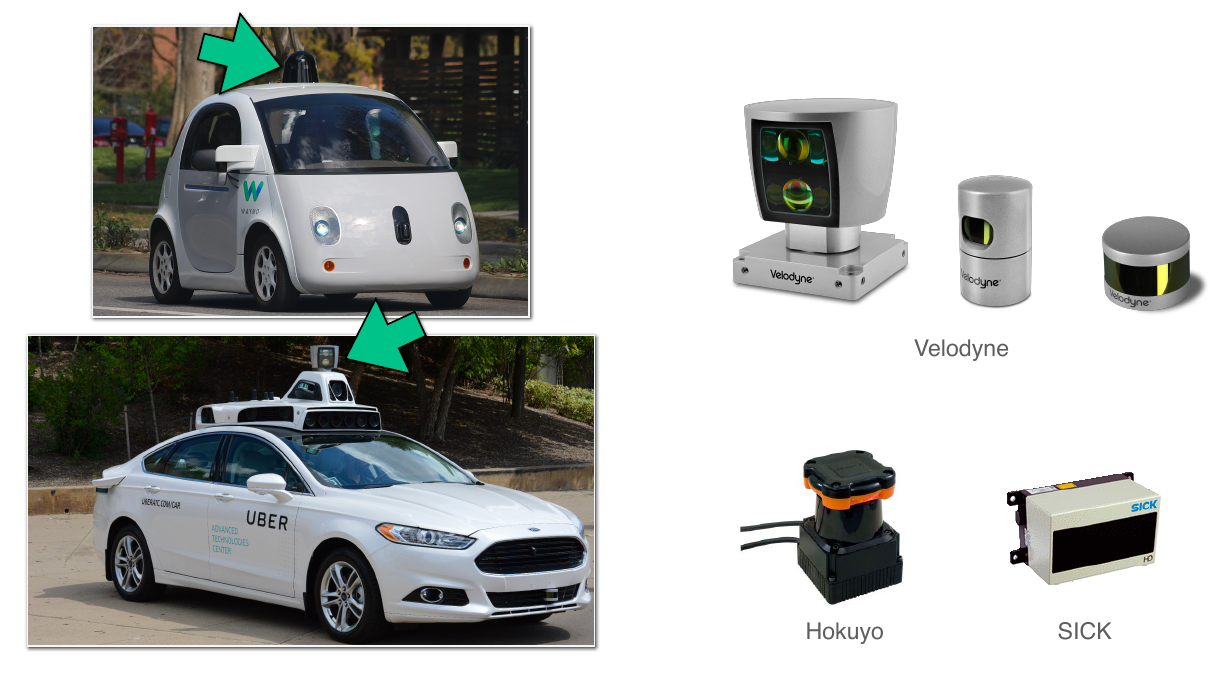
\includegraphics[scale=0.280]{img/hardware/lidar_1.jpeg}
\end{center}
\caption{Various types of LiDAR sensors.}
\label{lidar_1}
\end{figure}


In fact, LIDAR is one of the most common sensors used on self-driving cars and many other kinds of mobile robots. 
LIDARs come in many different shapes and sizes, and can measure the distances to a single point, 
a 2D slice of the world, or perform a full 3D scan. Some of the most popular models used today are manufactured by firms such
as Velodyne in California, Hokuyo in Japan, and SICK in Germany, see Figure \ref{lidar_1}. In this section, we will mainly focus on the Velodyne sensors as
our example of choice, but the basic techniques applied
to other types of LIDARs as well. 


\begin{framed}
\theoremstyle{remark}
\begin{remark}{\textbf{Some History}}

LIDAR was first introduced in the 1960s, not long after the invention
of the laser itself. The first group to use
LIDAR were meteorologists at the US National Center
for Atmospheric Research, who deployed LIDAR to measure
the height of cloud ceilings. These ground-based
celiometers are still in use today not only to
measure water clouds, but also to detect volcanic ash
and air pollution. Airborne LIDAR sensors are
commonly used today to survey and map the earth's
surface for agriculture, geology, military, and other uses. But the application that
first brought LIDAR into the public
consciousness was Apollo 15, the fourth manned mission
to land on the moon, and the first to use a laser altimeter
to map the surface of the moon. 
\end{remark}
\end{framed}

\subsection{LiDAR operating principles}

So, we've seen that LIDAR can be used to measure distances and create
a certain type of map, but how did they actually work, and how can we use them
onboard a self-driving car? To build a basic LIDAR in one dimension, you need three components:

\begin{itemize}
\item A laser
\item A photodetector
\item A very precise stopwatch
\end{itemize}

The laser first emits a short pulse of light usually in the near infrared frequency band
along some known ray direction. At the same time,
the stopwatch begins counting. The laser pulse travels
outwards from the sensor at the speed of light and
hits a distant target. Maybe another vehicle in
front of us on the road or a stationary object like
a stop sign or a building. As long as the surface of the target
is not too polished or shiny, the laser pulse will scatter off
the surface in all directions, and some of that reflected light will travel back along
the original ray direction. The photodetector catches that return
pulse and the stopwatch tells you how much time has passed between when the pulse first went out
and when it came back. That time is called the \textbf{round-trip} time. 

Further, we know the speed of light, which is a bit less than 300
million meters per second. So, we can multiply the speed of
light by the round-trip time to determine the total round trip distance
traveled by the laser pulse Figure \ref{lidar_3}. 

\begin{figure}[!htb]
\begin{center}
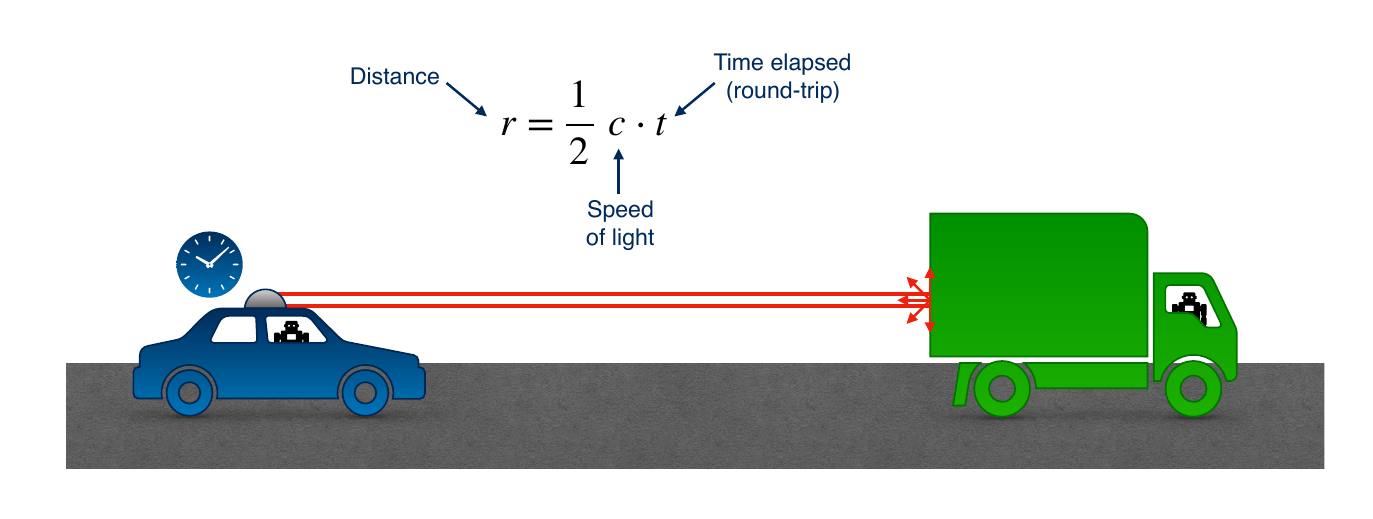
\includegraphics[scale=0.280]{img/hardware/lidar_3.jpeg}
\end{center}
\caption{Calculate distance with LiDAR.}
\label{lidar_3}
\end{figure}

Since light travels much faster than cars, it's a good approximation to think
of the LIDAR and the target as being effectively stationary
during the few nanoseconds that it takes for all of this to happen. That means that the distance from
the LiDAR to the target is simply half of the round-trip distance
we just calculated. This technique is called
\textbf{time-of-flight ranging}. Although it's not the only way
to build a LiDAR, it is a very common method
that also gets used with other types of ranging sensors like radar and sonar. 
It is worth mentioning that the photodetector also
tells you the intensity of the return pulse relative to the
intensity of the pulse that was emitted. This intensity information is less
commonly used for self-driving, but it provides some extra information
about the geometry of the environment and the material
the beam is reflecting off of. 

It is possible to create 2D images from LiDAR intensity data that
you can then use the same computer vision algorithms you'll
learn about in the next course. Since LiDAR is its own light source, it actually provides a way for
self-driving cars to see in the dark. 

We know how to measure a single distance to a single point using a laser, a photodetector, a stopwatch, and
the time-of-flight equation, but obviously it's not enough to stay laser focused on a single point ahead. 
How do we use this technique to measure a whole bunch of distances in 2D or in 3D?  The trick is to build
a rotating mirror into the LiDAR that directs the emitted pulses
along different directions. As the mirror rotates, you can measure distances at points
in a 2D slice around the sensor. If you then add an up
and down nodding motion to the mirror along with the rotation, you can use the same principle
to create a scan in 3D. For Velodyne type LiDARs, where the mirror rotates
along the entire sensor body, it's much harder to use
a knotting motion to make a 3D scan. 

Instead, these sensors will actually create multiple 2D scan lines from a series of individual lasers spaced at
fixed angular intervals, which effectively lets you paint the world with horizontal
stripes of laser light. Figure \ref{lidar_4} shows an example of
a typical raw LiDAR stream from a Velodyne sensor
attached to the roof of a car. 

\begin{figure}[!htb]
\begin{center}
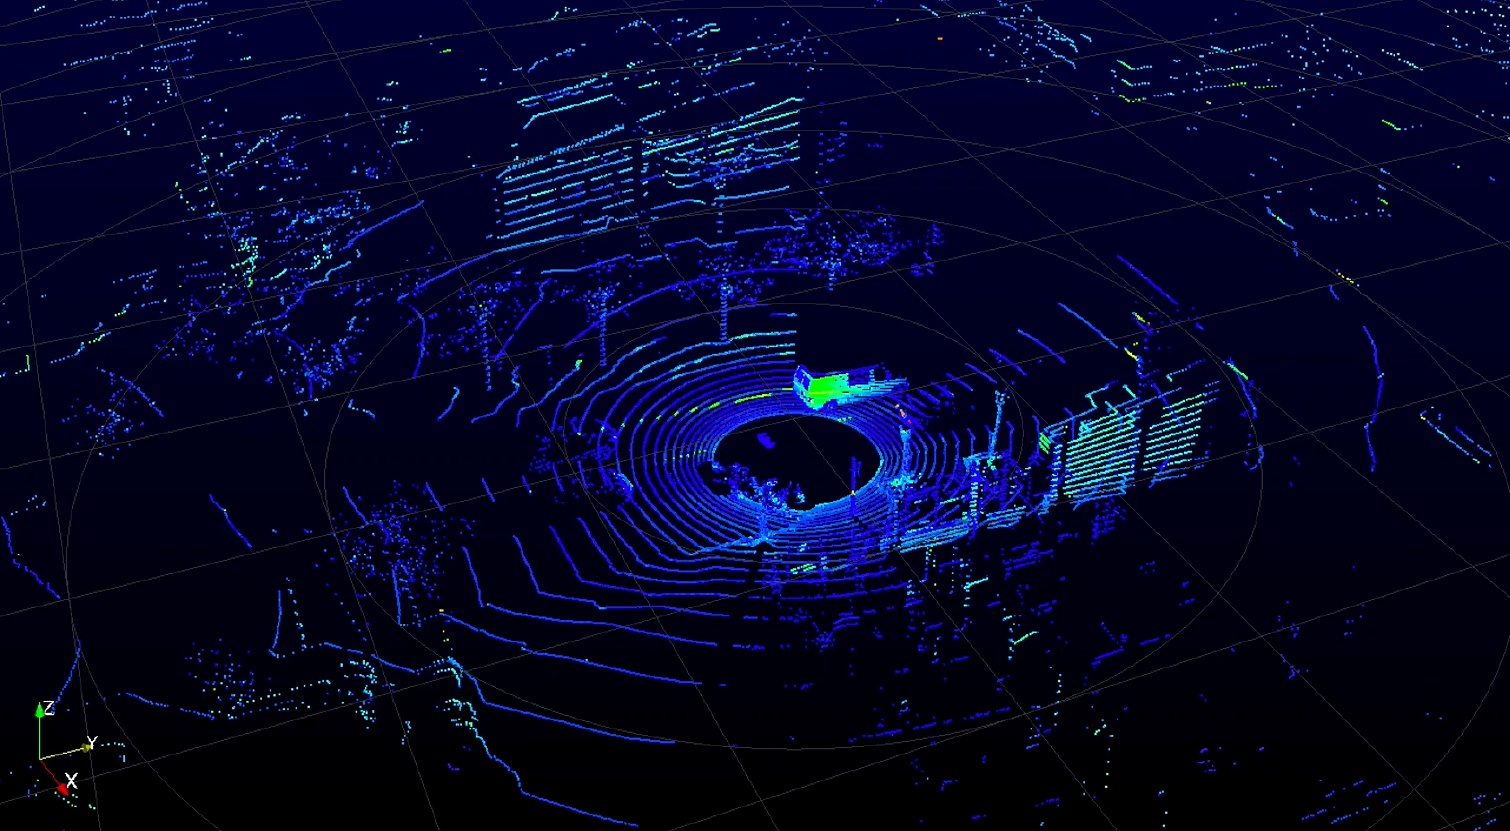
\includegraphics[scale=0.280]{img/hardware/lidar_4.jpeg}
\end{center}
\caption{Typical raw LiDAR stream.}
\label{lidar_4}
\end{figure}

The black hole in the middle is a blind spot where the sensor
itself is located, and the concentric circles
spreading outward from there are the individual scan lines produced
by the rotating Velodyne sensor. Each point in the scan is colored by
the intensity of the return signal. The entire collection of points in the 3D scan is called a point cloud. 

Now typically, LiDARs measure the position of points in 3D using
spherical coordinates, range or radial distance from
the center origin to the 3D point, elevation angle measured up
from the sensors $XY$ plane, and azimuth angle, measured
counterclockwise from the sensors $x$-axis. This makes sense because
the azimuth and elevation angles tell you the direction
of the laser pulse, and the range tells you how far in that direction
the target point is located. The azimuth and elevation angles
are measured using encoders that tell you
the orientation of the mirror, and the range is measured using the time
of flight as we've seen before. 


\begin{figure}[!htb]
\begin{center}
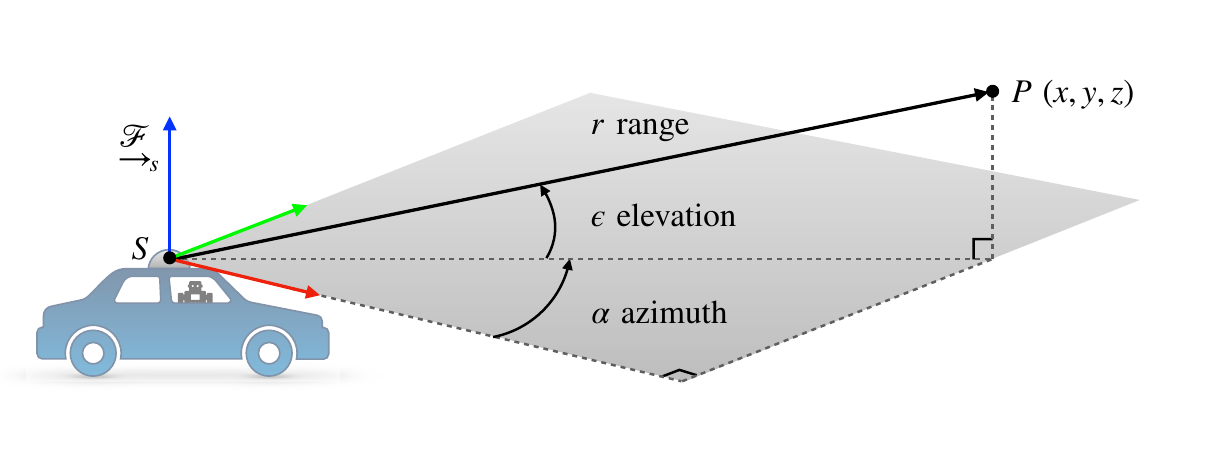
\includegraphics[scale=0.280]{img/hardware/lidar_5.jpeg}
\end{center}
\caption{Typical raw LiDAR stream.}
\label{lidar_5}
\end{figure}

\begin{framed}
\theoremstyle{remark}
\begin{remark}{}

For Velodyne type LIDARs, the elevation angle is fixed
for a given scan line.
\end{remark}
\end{framed}

Now, suppose we want to
determine the cartesian $XYZ$ coordinates of our scanned point
in the sensor frame, which is something we often
want to do when we are combining multiple LiDAR scans into a map. To convert from spherical
to Cartesian coordinates, we use the same formulas you would havve encountered in your mechanics classes. 

\begin{equation}
\begin{bmatrix}
x \\
y \\
z 
\end{bmatrix} = \mathbf{h}^{-1}(r, \alpha, \epsilon) = 
\begin{bmatrix}
r\cos(\alpha)\cos(\epsilon) \\
r\sin(\alpha)\cos(\epsilon) \\
\sin(\epsilon) 
\end{bmatrix} 
\label{lidar_inverse_sensor_model}
\end{equation}

This gives us an inverse sensor model. We say this is the inverse model because our actual measurements are
given in spherical coordinates, and we are trying to
reconstruct the Cartesian coordinates at the points
that gave rise to them. 

\begin{framed}
\theoremstyle{remark}
\begin{remark}{}

We can obviously get the forward model from the inverse model by using

\begin{equation}
\begin{bmatrix}
r \\
\alpha \\
\epsilon 
\end{bmatrix} = \mathbf{h}(x, y, z) = 
\begin{bmatrix}
\sqrt{x^2 + y^2 + z^2} \\
\arctan(\frac{x}{y}) \\
\arcsin(\frac{z}{\sqrt{x^2 + y^2 + z^2}} 
\end{bmatrix} 
\end{equation}

This is our forward sensor
model for a 3D LiDAR, which given a set of Cartesian coordinates defines what
the sensor would actually report.
\end{remark}
\end{framed}

Note that we have not said anything
about measurement noise yet. Most of the time the
self-driving cars we're working with use 3D LIDAR sensors
like the Velodyne, but sometimes you might want
to use a 2D LIDAR on its own, whether for detecting obstacles
or for state estimation in more structured environments
such as parking garages. Some cars have multiple 2D LiDARs strategically placed to
act as a single 3D LiDAR, covering different areas with a greater lesser density of measurements. 


\begin{framed}
\theoremstyle{remark}
\begin{remark}{\textbf{2D LiDAR}}

For 2D LIDARs, we use exactly the same forward and inverse sensor models. However, the elevation angle
enhance the $z$ component of the 3D point in the sensor frame are both zero. In other words, all of
our measurements are confined to the $XY$ plane of the sensor, and our spherical
coordinates collapsed to the familiar 2D polar coordinates. Figure \ref{lidar_6} summarizes the 2D case.
\end{remark}
\end{framed}

\begin{figure}[!htb]
\begin{center}
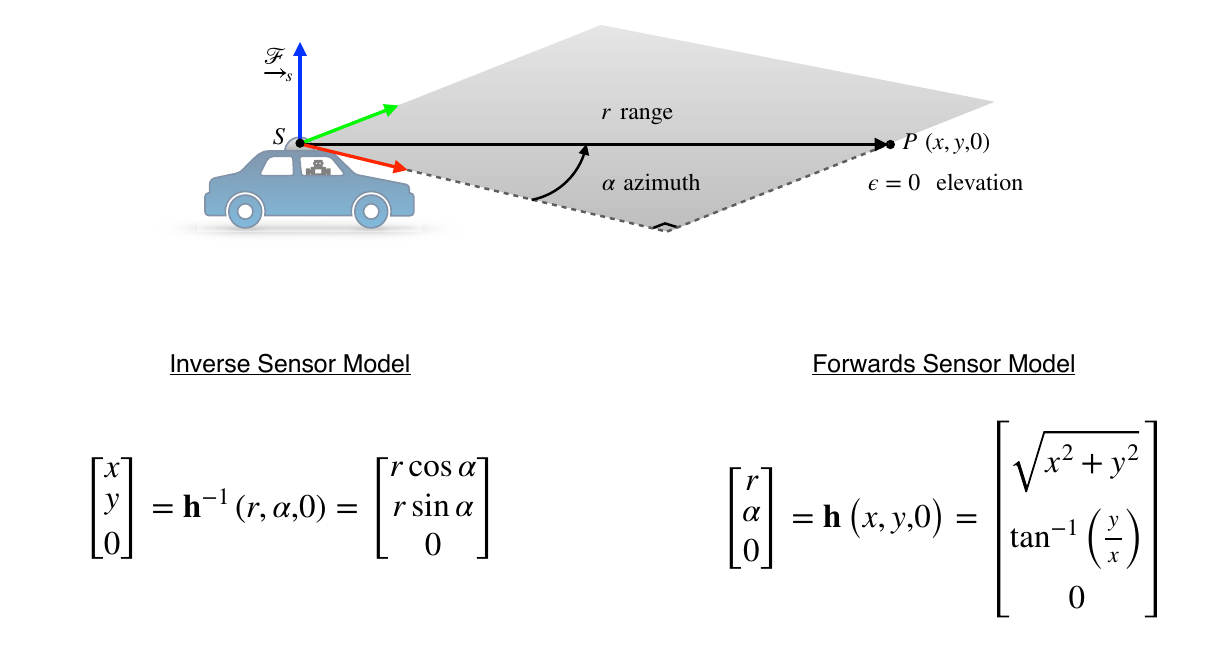
\includegraphics[scale=0.280]{img/hardware/lidar_6.jpeg}
\end{center}
\caption{2D LiDAR.}
\label{lidar_6}
\end{figure}

\subsection{Measurement noise}

We have seen now how to convert between spherical coordinates measured by the sensor and the cartesian coordinates that 
we will typically be interested in for state estimation, but what about measurement noise? For LiDAR sensors, there are several important sources
of noise to consider. First, there is uncertainty in the exact time of arrival of the reflected signal, which comes from the fact that
the stopwatch we use to compute the time of flight necessarily
has a limited resolution. Similarly, there is uncertainty in the exact orientation of the mirror in 2D and 3D LIDARs since the encoder is used to measure
this also have limited resolution. Another important factor
is the interaction with the target surface which can
degrade the return signal. For example, if the surface
is completely black, it might absorb most of the laser pulse. Or if it is very shiny like a mirror, the laser pulse might be scattered completely away from
the original pulse direction. In both cases, the LiDAR will typically
report a maximum range error, which could mean there is empty space
along the beam direction, or that the pulse encountered a highly absorptive or
highly reflective surface. In other words, you simply can not
tell if something is there or not, and this can be a problem for
safety if your self-driving car is relying on LiDAR alone to
detect and avoid obstacles. Finally, the speed of light actually varies depending on the material
it is traveling through. The temperature and humidity
of the air can also suddenly affect the speed of light in our
time-of-flight calculations for example. 

These factors are commonly accounted for by assuming additive zero-mean
Gaussian noise on the spherical coordinates with an empirically determined or
manually tuned covariance.  The Gaussian noise model is
particularly convenient for state estimation even if it is not
perfectly accurate in most cases. Another very important source
of error that can not be accounted for so easily
is motion distortion, which arises because the vehicle
the LiDAR is attached to is usually moving relative to
the environment it's scanning. Although the car is unlikely to be moving at an appreciable fraction
of the speed of light, it is often going to be moving at an appreciable fraction of
the rotation speed of the sensor itself, which is typically around 5-20 hertz when scanning objects at distances
of 10 to a 100 meters. This means that every single point
in a LiDAR sweep is taken from a slightly different position and
a slightly different orientation, and this can cause artifacts such as duplicate objects to
appear in the LIDAR scans. This makes it much harder for a self-driving car to
understand its environment, and correcting this motion
distortion usually requires an accurate motion model for the vehicle provided by GPS and INS for example. 

\subsection{Summary}

To recap, LIDAR sensors
measure distances by emitting pulse laser light and measuring
the time of flight of the pulse. 2D or 3D LIDAR is extend
this principle by using a mirror to sweep the laser across the environment and measure distances in many directions. We will look more closely at the point
clouds created by 2D and 3D LIDARs, and how we can use them for state estimation on-board our self-driving car.

\section{LiDAR sensor model and point clouds}
\label{lidar_and_point_clouds}

In section \ref{lidar_principles}, we talked about the basic operating principles of LiDAR, one of the most popular sensor choices for
self-driving cars. In the next two sections we will learn how we
can use the point cloud generated by LiDAR sensors to do state estimation for
our self-driving car. 

By the end of this section, you'll be able
to describe the basic point cloud data structure used to store LiDAR scans. Describe common spatial operations on
point clouds such as rotation and scaling. Use the method of least squares to
fit a plane to a point cloud in order to detect the road or other surfaces. 

To begin with, recall that a 3D LIDAR sensor returns measurements of range, elevation angle, and azimuth angle for
every point that it scans. We know how to convert these spherical
coordinates into Cartesian $x, y, z$ coordinates using
the inverse sensor model, see equation \ref{lidar_inverse_sensor_model} so we can build up a large point cloud using
all the measurements from a LiDAR scan. For some LiDAR setups, it is not uncommon for these point clouds to contain
upwards of a million points or more. 

So what can we do these massive point clouds? Let us consider an example of a point cloud
we might encounter in the real world. Let us say our LIDAR scans a nearby
tree off on the side of the road, and produces a point cloud
that looks like this. 


\begin{figure}[!htb]
\begin{center}
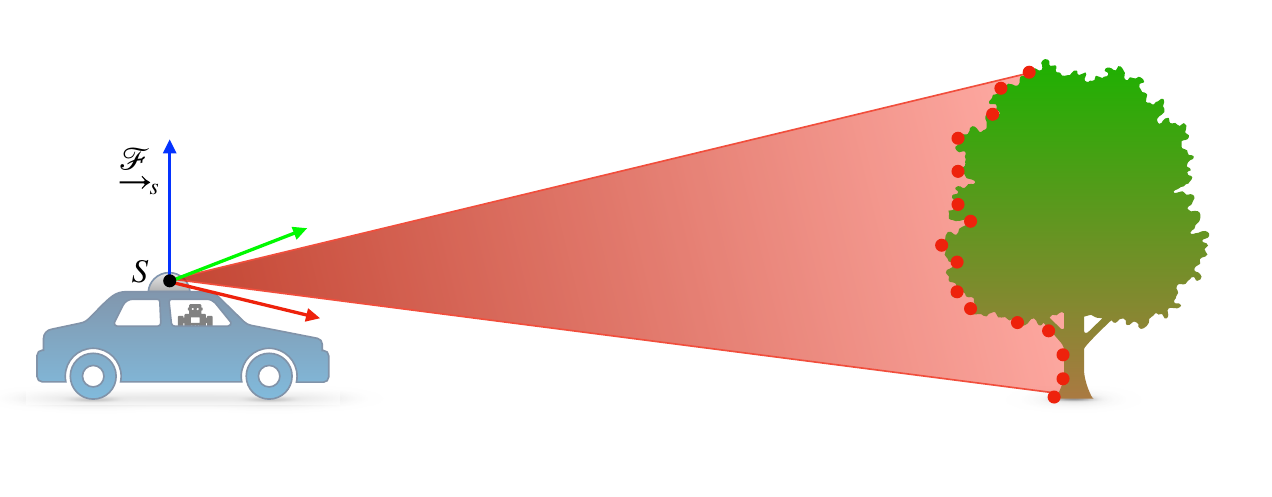
\includegraphics[scale=0.280]{img/hardware/lidar_7.jpeg}
\end{center}
\caption{Assumed LiDAR scan.}
\label{lidar_7}
\end{figure}

We only see points on the part of the tree
that is facing us because the tree and the leaves reflect infrared light. The first question you might ask is how
do we keep track of all of these points? What kinds of data structures
should we use to work with them? One common solution is to assign
an index to each of the points, say point 1 through point $n$,
and store the $x, y, z$  coordinates of each point
as a 3 by 1 column vector. From there, you could think about storing
each of these vectors in a list, or you could stack them side by side
into a matrix that we'll call $\mathbf{P}$. Doing it this way make it easier to
work with the standard linear algebra libraries, like the Python NumPy library,
which lets us take advantage of fast matrix operations rather than
iterating over a list and treating each vector independently. So what kind of operations
are we talking about? 

There are three basic spatial
operations that are important for carrying out state estimation with point clouds. 

\begin{itemize}
\item Translation
\item Rotation
\item Scaling
\end{itemize}

We will talk about each of these in turn. When we think about spatial
operations on point clouds, our intuition might be to think in terms
of physically manipulating the point cloud while our reference frame stays fixed. But for state estimation, it's more useful to think about
things the other way around. Objects in the world mostly stay
put while the reference frame attached to the vehicle moves and observes
the world from different perspectives. 

\subsection{Basic spatial operations}

So let's think about how translating our
reference frame, say, by driving for a ten meters will affect our perception
of a single point in point cloud. 

We can start by drawing the vector from the origin of our sensor frame, $S$, to a point, $P$. Now, consider a second frame, $S^{'}$, whose origin has been translated relative
to $S$ due to motion of the vehicle, see Figure \ref{lidar_8}. 


\begin{figure}[!htb]
\begin{center}
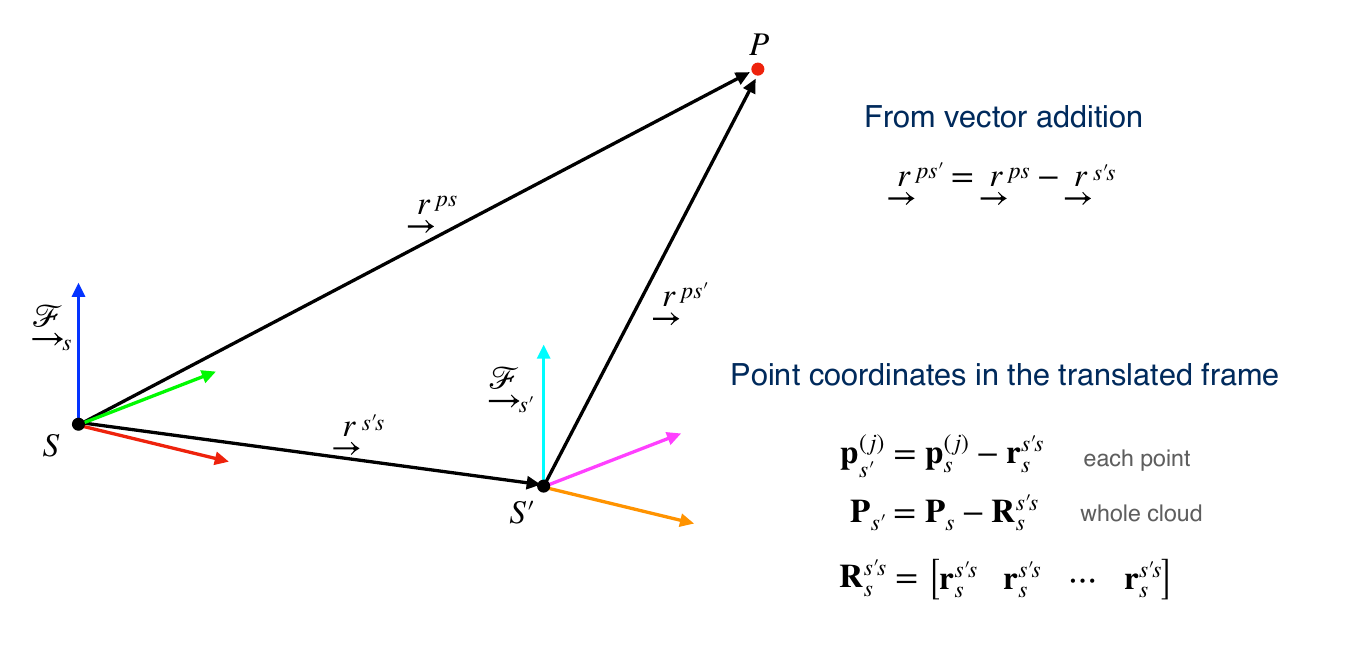
\includegraphics[scale=0.280]{img/hardware/lidar_8.jpeg}
\end{center}
\caption{Translation operation.}
\label{lidar_8}
\end{figure}

Note that the basis vectors of frame $S^{'}$ are the same as the basis vectors of frame $S$. Only the origin has moved. We can draw another vector from
the origin of $S^{'}$ to the point $P$. Immediately, we notice the resulting vector, indicated here, is just the tip to
tail sum of the other two vectors, see Figure \ref{lidar_8}. These vectors are just geometric
objects until we express them in a coordinate system. What we are after are the coordinates
of the point $P$ in frame $S^{'}$. We can get these easily by just subtracting the frame-to-frame translation vector from
the coordinates of $P$ in frame $S$. This extends easily to a batch operation
on the full point cloud by simply tiling the frame-to-frame translation
in a big matrix $\mathbf{R}$, and subtracting it from
the point cloud matrix. 

\begin{framed}
\theoremstyle{remark}
\begin{remark}{}

Depending on the language or
linear algebra library you are using, you probably will nott need to
build this $\mathbf{R}$ matrix explicitly. In Python, for example, the NumPy
library is smart enough to repeat the frame-to-frame translation
implicitly using broadcasting semantics.
\end{remark}
\end{framed}

Now, let's think about what happens if rotate our reference frame instead of translating it. Again, keep in mind that we're not
changing the physical point $P$, only our view of it. So in this case, we only have to think about one vector
from the origin of frame $S$ to $P$. What does change in this case is actually
the set of basis vectors we use to express the coordinates
of the vector $S$ to $P$. Remember that the rotation matrix $\mathbf{C}$ tells
us how to find the coordinates of a vector in a rotated frame from the coordinates
of the vector in the original frame. Thus, if we know the rotation matrix
from frame $S$ to frame $S^{'}$, all we have to do is multiply it
against the coordinates of $P$ in frame $S$ to get the coordinates
of $P$ in frame  $S^{'}$. To determine the coordinates of the entire
rotated point cloud, the operation is exactly the same, thanks to
the properties of matrix multiplication. 

\begin{equation}
\mathbf{P}_{S^{'}} = \mathbf{C}_{S^{'}S} \mathbf{P}_{S}
\end{equation}

The last spatial operation
to think about is scaling, which works very similarly to rotation. But instead of changing the direction
of the basis vectors in our coordinate system,
we're changing their lengths. Mathematically, this just means
pre-multiplying the coordinates of each point by a diagonal matrix
$\mathbf{S}$ whose non-zero elements are simply the desired scaling
factors along each dimension. Often but not always these
scaling factors are the same, and the matrix multiplication is
equivalent to multiplying by a scalar. In these cases, we say that the scaling
is isotropic or equal in every direction. We can use the same matrix multiplication
for individual points or for the entire point cloud,
just like we did for rotations.

Usually, the transformations we're interested in are a combination of translation and rotation and
sometimes scaling. For example, we are often interested
in estimating the translation and rotation that best aligns
to point clouds so that we can estimate the motion
of our self-driving car. Fortunately for us, it's easy to combine
all three operations into a single equation By first translating each vector, then rotating into the new frame,
and finally applying any scaling. Of course, this operation
extends to the batch case as well. So we have seen how to apply basic
spatial operations to point clouds. 

\subsection{Plane fitting}
\label{plane_fitting}

One of the most common and important applications of plane-fitting for self-driving cars is figuring out
where the road surface is and predicting where it is going to
be as the car continues driving. If you think back to your
high school geometry classes, you might remember
the equation of a plane in 3D. 

\begin{equation}
z = a + bx +cy
\end{equation}

This equation tells you how the height of the plane $z$ changes as you move around in the $x$ and
$y$ directions. It depends on three parameters, $a, b$, and $c$, which tells you the slope of the plane in each direction and
where the $z$ axis intersects the plane. So in our case, we have a bunch
of measurements of $x, y$ and $z$ from our LIDAR point cloud, and we
want to find values for the parameters $a, b$, and $c$ that give us the plane
of best fit through these points. To do this, we are going to use least-squares estimation. We will start by defining a measurement
error $e$ for each point in the point cloud. $e$ is just going to be the difference
between the predicted value of our dependent variable $\hat{z}$  and
the actual observed value of $z$. 


\begin{equation}
e_j = \hat{z}_j - z_j  = \hat{a} + \hat{b}x + \hat{c}y - z_j, j=1, \ldots, n
\end{equation}


We get $\hat{z}$ simply by plugging our
current guess for the parameters $\hat{a}$ , $\hat{b}$, and $\hat{c}$, and
the actual values of $x$ and $y$ in. In this case, the error, $e$, that we are
considering, is for a bumpy road surface, for example.  Note that for the moment, we are ignoring the actual
errors in the LiDAR measurements themselves, which also have an effect. 


We can stack all of these error terms into matrix form so we have a big matrix of
coefficients called $\mathbf{A}$. Multiplied by our parameter vector $\mathbf{x}$,
minus our stack measurements $\mathbf{b}$. 

\begin{equation}
\underbrace{\begin{bmatrix}
e_1 \\
e_2 \\
\vdots \\
e_n
\end{bmatrix}}_{\mathbf{e}} = 
\underbrace{\begin{bmatrix}
1 & x_1 & y_1 \\
1 & x_2 & y_2 \\
\vdots & \vdots & \vdots \\
1 & x_n & y_n
\end{bmatrix}}_{\mathbf{A}}
\underbrace{\begin{bmatrix}
a \\
b \\
c
\end{bmatrix}}_{\mathbf{x}} -
\underbrace{\begin{bmatrix}
z_1 \\
z_2 \\
\vdots \\
z_n
\end{bmatrix}}_{\mathbf{b}}
\end{equation}


You can work out the matrix multiplication yourself to see that we get back the same measurement error
equations we started out with. 

Now, all we have to do is minimize
the square of this error and we will have our solution. We can start by multiplying out
the square to get a matrix polynomial in the parameter vector $\mathbf{x}$. From there, we take the partial derivative
of the squared error function with respect to the parameter vector $\mathbf{x}$ and
set it to 0 to find the minimum. This gives us the linear system we will
need to solve to obtain the final least squares estimate. 

\begin{equation}
\hat{\mathbf{x}} = (\mathbf{A}^T\mathbf{A})^{-1}\mathbf{A}^T\mathbf{b}
\end{equation}


We can solve this linear system using
an efficient numerical solver like Python NumPy's solve function. Or just use the pseudo inverse to get our
final answer for the plane parameters. 

One important thing to notice here is that we did not account for sensor noise in our $x, y, z$ measurements. All we did was to find the plane
of best fit through a set of points. It is certainly possible to set this
problem up in a more sophisticated way that does account for sensor noise. You could use a batch approach
similar to what we just discussed, or you could even think about including the
road parameters in the column filter to estimate them on the fly as
the sensor data comes in. 

The best solution for your self-driving application will depend
on how much you trust your LiDAR data and how much thought you want to give
to uncertainty in the road surface. Now, although all of the operations we've
described here can be easily implemented with NumPy or any other linear algebra library, there is a fantastic open source tool
called the Point Cloud Library, or PCL, that provides all sorts of useful
functions for working with point clouds. In fact, it is so useful that you'll
find it everywhere in industry. The core library is built with C++, but there are unofficial Python
bindings available as well. If you want to learn more
about the features PCL.

\subsection{Summary}

In summary, we have seen that point
clouds are a way of capturing all of the measurements from a LiDAR scan. They are often stored as a big matrix. We saw how we can use linear algebra to
do useful operations on point clouds, like translating, rotating, and scaling. We also saw how we can use
the least squares algorithm to fit a 3D plane to a point cloud
to find the road surface. The Point Cloud Library, or PCL,
implements a bunch of useful tools for working with point clouds in C++. One of the most useful algorithms in PCL
is called the iterative closest point algorithm, or ICP,
which is a common method for estimating the motion of a self-driving
car using two LIDAR point clouds. 


\section{Pose estimation from LiDAR data}

In this section, we will talk
about how we can actually use these operations with real point clouds to estimate the motion of
a self-driving car. The way that we do this in general is by solving something called the point set
registration problem, which is one of
the most important problems in computer vision and
pattern recognition. 

By the end of this section, you will be able to
describe the point set registration problem and how it can be used for
state estimation, describe and implement the Iterative Closest Point or ICP algorithm for
point set registration, and understand some
common pitfalls of using ICP for state estimation
on self-driving cars. 

\subsection{The point set registration problem}
\label{point_set_registration_problem}

Let us explore this problem by returning to our example of a self-driving car observing a tree from a LIDAR
mounted on the cars roof. At time $t=1$ say, the LiDAR returns
a point cloud that follows the contour of
the tree as before.  The coordinates of every point in the point cloud are given relative to the pose of the lidar at the time
of the scan, we will call this
coordinate frame $S$. At time $t=2$ the car is
driven a bit further ahead, but the LiDAR can
still see the tree and return a second point cloud whose coordinates are again
specified relative to the pose of the lidar
at time t equals two, we will call this
coordinate frame $S^{'}$. Now, the point set
registration problems says, given two point clouds in
two different coordinate frames, and with the knowledge that they correspond to or contain the same object
in the world, how shall we align them to
determine how the sensor must have moved
between the two scans? More specifically,
we want to figure out the optimal translation and the optimal rotation between the two sensor
reference frames that minimizes the distance
between the 2 point clouds. To keep things simple, we are going to pretend that
we have an ideal LiDAR sensor that measures the entire point
cloud all at once, so that we can ignore the
effects of motion distortion. Now, if we somehow knew that
each and every point in the second point
cloud corresponded to a specific point in
the first point cloud, and we knew ahead of time which points
corresponding to which, we could solve this
problem easily. All we would have to do is
find the translation and rotation that lines up
each point with its twin. 

In this example, our ideal rotation matrix would be the identity matrix, that is no rotation at all, and a ideal translation would be along the cars forward direction. The problem is
that, in general we do not know which points
correspond to each other.  Feature matching which is one way of determining correspondences between
points using camera data. For now let us think
about how we might solve this problem without knowing any of the correspondences
ahead of time. The most popular algorithm for solving this kind of
problem is called the Iterative Closest Point
algorithm or ICP for short. 

\subsection{Iterative closest point}

The basic intuition behind ICP is this, when we find the optimal
translation and rotation, or if we know something
about them in advance, and we use them to transform one point cloud into the
coordinate frame of the other, the pairs of points that truly correspond to each other will be the ones that are closest to each other in a Euclidean sense. This makes sense if you consider the simplified case where our LiDAR sensors scans exactly the same points just from two different
vantage points. In this case, there is a one-to-one mapping between points
in the two scans, and this mapping is completely determined by the motion
of the sensor. 

This is  the ideal case for when we found the best possible
translation and rotation, but what if we do not have the optimal translation
and rotation, how do we decide which points
actually go together? Well, with ICP we use
a simple heuristic, and say that for
each point in one cloud, the best candidate for
a corresponding point in the other cloud is the point that is closest to it right now. The idea here is
that this heuristic should give us
the correspondences that let us make our next guess for the translation and rotation, that is a little bit better
than our current guess. As our guesses get
better and better, our correspondences should also get better and better until we eventually converge
to the optimal motion and the optimal correspondences. 

This iterative optimization scheme using the closest point heuristic
is where ICP gets its name. It is important to
note that the word closest implies that we
will find points that lie close together after applying the frame to
frame transformation only. This is, because the vehicle is moving it is almost never the case that a laser beam will hit exactly the same
surface point twice. 

Let us now talk about the steps
in the ICP algorithm. First and most
important is that we need an initial guess
for the transformation. 

\begin{equation}
\check{\mathbf{C}_{S^{'}S}}, \check{\mathbf{r}_{S}^{S^{'}S}} 
\end{equation}


We need this because there is no guarantee that the closest point heuristic will actually converge to
the best solution. It's very easy to get stuck in a local minimum in these kinds of
iterative optimization schemes. So, we will need
a good starting guess. 

Now, the initial guess can come from a number of sources. One of the most
common sources for robotics applications
like self-driving is a motion model, which could be
supplied by an IMU or by wheel odometry or
something really simple like a constant velocity or
even a zero velocity model. How complex the motion model
needs to be to give us a good initial guess really depends on how smoothly
the car is driving. If the car is moving
slowly relative to the scanning rate
of the LIDAR sensor, one may even use the last known pose
as the initial guess. For our example, let's say we use a very noisy IMU and emotion model to provide
the initial guess. The model tells us that
the sensor translated forward a bit and
also pitched upwards. In step two, we will use
this initial guess to transform the coordinates of the points in one cloud into the reference
frame of the other, and then match each point in the second cloud to the closest
point in the first cloud. 


\begin{figure}[!htb]
\begin{center}
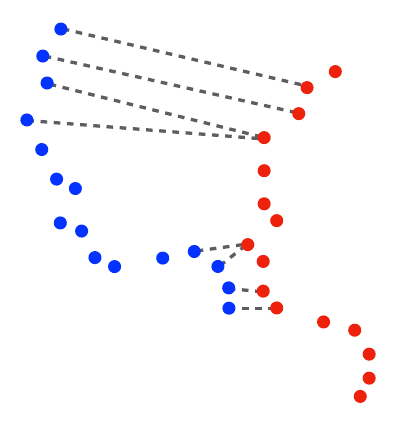
\includegraphics[scale=0.280]{img/hardware/lidar_9.jpeg}
\end{center}
\caption{Associate each point in $\mathbf{P}_{S^{'}}$ with the nearest point in $\mathbf{P}_{S}$.}
\label{lidar_9}
\end{figure}

Figure \ref{lidar_9} shows
the associations for the first four points and
the last four points. Note that there's nothing
stopping two points in one cloud from being
associated with the same point in
the other cloud. 

Step three is to take all of those match points and find
the transformation that minimizes the sum of squared distances between
the corresponding points. You can visualize
it as wrapping an elastic band around
each pair of matched points, and then letting go and
waiting for the system to find its lowest
energy configuration. The translation and
rotation associated with this minimum energy configuration are the optimal solutions. Then, we repeat the process
using the translation and rotation we just solved for
as our new initial guess. We keep going until
the optimization converges. Thus, in the next iteration, we use the new translation
and rotation to transform the point cloud and then
find the closest matches, solve for the optimal
transformation, and keep going until we reach the optimum after a few iterations. 


How do we actually solve for the optimal transformation
in step three? One option is to use least-squares. Our goal here is to
find the rotation and translation that best aligns
the two point clouds. Specifically, you want
to minimize the sum of squared euclidean
distances between each pair of matched points, which is one of the loss function that we've defined here. 


\begin{equation}
{\check{\mathbf{C}}_{S^{'}S}, \check{\mathbf{r}}_{S}^{S^{'}S}} = argmin_{\mathbf{C}_{S^{'}S}, \mathbf{r}_{S}^{S^{'}S}} L_{LS}(\mathbf{C}_{S^{'}S}, \mathbf{r}_{S}^{S^{'}S}) 
\end{equation}

This least squares problem
is a little bit more complex. This is because
the rotation matrix is inside the loss function. It turns out the
rotation matrices do not behave like vectors. If you add two vectors together, you get another vector. But if you add two
rotation matrices together, the result is not necessarily
a valid rotation matrix. In reality, 3D rotations
belong to something called the special orthogonal group or SO3. 

It turns out that there is a nice closed form solution to this least-squares
problem which was discovered in the 1960s. We will not  go through
the derivation here, but the good news
is that there is a simple four step algorithm you can follow to
solve this problem. The first two steps are easy. First, we compute the centroid of each point cloud by taking the average over
the coordinates of each point. This is exactly like calculating the center of mass in physics. 

\begin{equation}
\boldsymbol{\mu}_S = \frac{1}{n} \sum_{j=1}^{n} \mathbf{p}_{S}^{j}, ~~ \boldsymbol{\mu}_{S^{'}} = \frac{1}{n} \sum_{j=1}^{n} \mathbf{p}_{S^{'}}^{j}
\end{equation}

Second, we work at a three-by-three matrix capturing the spread of
the two point clouds. 

\begin{equation}
\mathbf{W}_{S^{'}S} = \frac{1}{n} \sum_{j=1}^{n} (\mathbf{p}_{S}^{j} - \boldsymbol{\mu}_S) (\mathbf{p}_{S^{'}}^{j} - \boldsymbol{\mu}_{S^{'}})^T
\end{equation}

You can think of this $\mathbf{W}$ matrix
as something like an inertia matrix you might
encounter in mechanics. The $\mathbf{W}$ matrix is the quantity
we are going to use to estimate the optimal
rotation matrix. 

Step three is actually finding the optimal rotation matrix. This step is the most complex, and it involves taking
something called the singular value decomposition
or SVD of the $\mathbf{W}$ matrix. 

\begin{framed}
\theoremstyle{remark}
\begin{remark}{\textbf{Singular Value Decomposition or SVD}}

The SVD is a way of factorizing a matrix into the product
of two unitary matrices, $\mathbf{U}$ and $\mathbf{V}$, and a diagonal matrix $\mathbf{D}$, whose non-zero entries
are called the singular values of the original matrix. 

\begin{equation}
\mathbf{W}_{S^{'}S} = \mathbf{U}\mathbf{D}\mathbf{V}^T
\end{equation}
\end{remark}
\end{framed}

There are several ways to interpret the SVD. For us, it is easiest
to think about $\mathbf{U}$ and $\mathbf{V}$ as rotations and the $\mathbf{D}$ matrix
as a scaling matrix. Since we are dealing with rigid body motion in this problem, we do not want any scaling
in a rotation estimate, so we will replace
the $\mathbf{D}$ matrix with something like the identity matrix
to remove the scaling. 

\begin{equation}
\mathbf{D} = 
\begin{bmatrix}
1 & 0 & 0 \\
0 & 1 & 0 \\
0 & 0 & \text{det}\mathbf{U}\text{det}\mathbf{V}
\end{bmatrix}
\end{equation}

It turns out that in some cases, the SVD will give us rotation matrices that
are not proper rotations. That is, they also have a reflection about
the axis of rotation. To make sure that we
get a proper rotation, we choose the bottom
right term to be the product of
the determinants of $\mathbf{U}$ and $\mathbf{V}$. This number will be either plus one or minus one and will
cancel out any reflection. Once we have this,
all we have to do is multiply out the three matrices. This gives us back
the optimal rotation matrix. 

Now, that we have our rotation estimate, the last step is to
recover the translation. 

\begin{equation}
\hat{\mathbf{r}}_{S}^{S^{'}S} = \boldsymbol{\mu}_S - \check{\mathbf{C}}_{S^{'}S}^T \boldsymbol{\mu}_{S^{'}}, ~~ \check{\mathbf{C}}_{S^{'}S} = \mathbf{U}\mathbf{D}\mathbf{V}^T
\end{equation}

This part is very straightforward and only involves rotating the centroid of one point cloud into
the reference frame of the other and then
taking the difference of the coordinate vectors to find the translation that will best align the two point clouds. 

One other important thing to think about, both from a safety standpoint
and when we start talking about sensor fusion, is how confident we should be in the output of the ICP algorithm. There are a number
of different ways to estimate the uncertainty or the covariance of
the estimated motion parameters. An accurate and
relatively simple method is to use this equation here. 

\begin{equation}
\text{cov}(\hat{\mathbf{x}}) \approx
\begin{bmatrix}
(\frac{\partial^2 L}{\partial \mathbf{x}^2})^{-1}, \frac{\partial^2 L}{\partial \mathbf{z}\partial\mathbf{x}}, \frac{\partial^2 L}{\partial \mathbf{z}\partial\mathbf{x}}(\frac{\partial^2 L}{\partial \mathbf{x}^2})^{-1} 
\end{bmatrix}_{\mathbf{x} = \hat{\mathbf{x}}}
\end{equation}

This expression tells us
how the covariance of the estimated motion parameters is related to the covariance of the measurements in
the two point clouds using certain second-order
derivatives of the least squares cost function. While its expression is
accurate and fast to compute, it's a little tricky to derive these second-order
derivatives when there's a constraint quantity like
a rotation matrix in the mix. For our purposes, we're
generally going to hand tune the ICP covariance matrix to
give us acceptable results. 

\subsubsection{ICP variants}

You have now seen
the basic vanilla algorithm for the iterative
closest point method, but it's not the only way
of solving a problem. In fact, this algorithm is just one variant of ICP
called Point-to-point ICP, which derives its name from the fact that
our objective function or loss function
minimizes the distance between pairs of
corresponding points. 

Another popular variant that works well in unstructured
environments like cities or indoors is
called Point-to-plain ICP. Instead of minimizing
the distance between pairs of points, we fit a number of planes to the first point cloud and
then minimize the distance between each point in the second cloud and its closest plane
in the first cloud. These planes could
represent things like walls or road surfaces. The challenging part
of the algorithm is actually figuring out
where all the planes are. You can check out
the documentation for Point-to-plain ICP in the point cloud library
for more information. 

\subsection{Objects in motion}

Now, up until this point, we've been assuming
that the objects seen by our LiDAR are stationary. What
if they're moving? A common example of this is
if our car is driving in traffic down a busy highway and scanning the vehicle
in front of it. Both vehicles are traveling
at the same speed while our self-driving car is happily collecting LiDAR data points. We ask ourselves again, what motion of the car best
aligns the two point clouds? The answer we get is that
we haven't moved at all. But, of course, we did move, just not relative to the vehicle
directly ahead of us. This is obviously
a contrived example. In reality, the point
cloud would also include many stationary
objects like roads, and buildings, and trees. But naively using ICP in
the presence of moving objects will tend
to pull our motion estimates away from
the true motion. So we need to be
careful to exclude or mitigate the effects of
outlying points that violate our assumptions
of a stationary world. One way to do this is
by fusing ICP motion estimates with GPS
and INS estimates. Another option is to identify
and ignore moving objects, which we could do with some
of the computer vision. An even simpler
approach for dealing with outliers like these is to choose a different loss function that is less sensitive to large errors induced by outliers than our standard
squared error loss. The class of loss functions that have this
property are called \textbf{Robust Loss Functions} or
robust cost functions, and there are several
to choose from. We can write this
out mathematically by generalizing our least squares loss function so that
the contribution of each error is not simply
the square of its magnitude, but rather, some
other function $\rho$. Some popular choices for
robust loss functions include the Absolute
error or L1 norm, the Cauchy loss, and
the Huber loss are shown in Figure \ref{lidar_10}. 

\begin{figure}[!htb]
\begin{center}
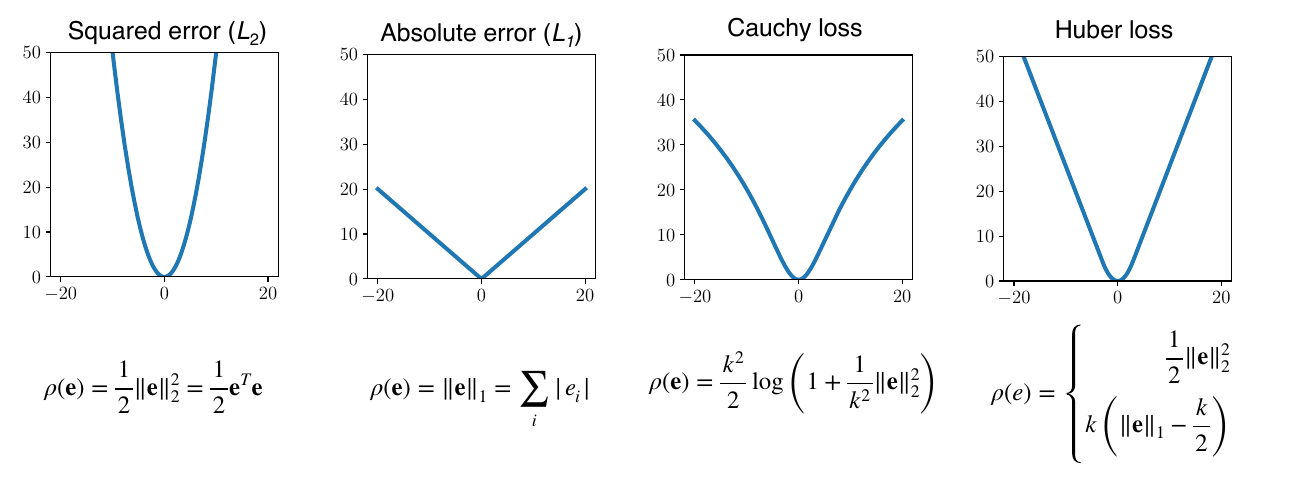
\includegraphics[scale=0.280]{img/hardware/lidar_10.jpeg}
\end{center}
\caption{Robust Loss Functions.}
\label{lidar_10}
\end{figure}

The key difference is that the slope of the
loss function does not continue to increase as
the errors become larger, but rather, it remains
constant or it tapers off. Robust loss functions make the ICP problems slightly
more difficult because we can no longer derive
a nice closed form solution for the point cloud
alignment step, and this means we need to add another iterative optimization
step inside our main loop. However, the benefits cannot
weigh the added complexity. 

\subsection{Summary}

In summary, the Iterative
Closest Point or ICP algorithm is
a way to determine the motion of
a self-driving car by aligning point clouds from
LiDAR or other sensors. ICP works by iteratively minimizing the Euclidean
distance between neighboring points
in each point cloud which is where the algorithm
gets its name. Moving objects can be
a problem for ICP since they violate the stationary
world assumption that ICP is based on. Outlier measurements like these can be mitigated with a number of techniques including
Robust Loss Functions, which assign less weight to large errors than
the usual squared error loss.


\section{The inertial measurement unit IMU}
\label{inertial_measurement_unit}

In this section we are going to discuss the Inertial Measurement Unit or IMU. By the end of this section you should be able
to 

\begin{itemize}
\item Describe the operating principles of the two sensors that make up the basic
IMU, an Accelerometer and a Gyroscope. 
\item Model each of these sensors, and account for things like sensor noise and bias. This will be crucial when we incorporate
an IMU into a full-state estimator. 
\end{itemize}



The inertial measurement unit, or IMU measures the movement of
a body in inertial space. Today a certain type of cheap,
mass manufactured IMU, is found in nearly every smartphone,
such as the iPhone X shown in Figure \ref{iphone_x}. 


\begin{figure}[!htb]
\begin{center}
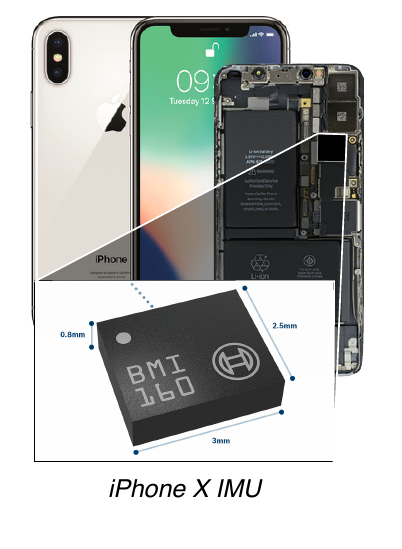
\includegraphics[scale=0.280]{img/hardware/iphone_x.jpeg}
\end{center}
\caption{iPhone X IMU.}
\label{iphone_x}
\end{figure}


Despite their ubiquity today, the development of a sensor that
could accurately track the motion of a moving body was a significant
achievement of the 20th century. The IMU aided transoceanic flights long
before GPS, and was crucial to the Apollo missions as part of the on board guidance,
navigation, and control system. The Apollo spacecraft relied on an IMU
to accurately track both the position, and orientation of the vehicle
on the long voyage to the moon. In space, there are few landmarks
to rely on for guidance. One can track the fixed stars but
this is not easy. The onboard IMU which
operated without the need for such landmarks enabled safe
navigation to the Moon's surface. In modern self-driving cars,
IMUs play a very similar role.  

Generally, an inertial measurement
unit is a composite sensor suite that combines 

\begin{itemize}
\item Three gyroscopes 
\item Three accelerometers 
\end{itemize}

in order to track the exterior
free movement of a rigid body. Some IMUs also incorporate magnetometers,
or a compass, to help track orientation. IMUs come in many shapes and forms. The sensors found in modern
smartphones are relatively cheap, often costing less than a few
dollars when purchased in bulk. They are lightweight and
require relatively little power but produce quite noisy measurements. More expensive IMUs use more complex
components and have more accurate calibration models that can remove the
effects of temperature fluctuations, for example. Let's discuss the components of an IMU. 

\subsection{Gyroscope}

The gyroscope has a long history. The term gyroscope can be quite confusing,
because it refers to several concepts all relating to the idea of measuring
orientation or change in orientation.  Historically, a gyroscope was
a spinning disk that due to its angular momentum resisted
changes in orientation. In the late 19th and early 20th century,
engineers realized that this spinning wheel could be used as
an orientation reference for marine and aeronautical navigations. 

This required precise machining,
and instead of gimbals, it used high quality jewel or
numeric bearings. Although this type of spinning disc
gyroscope can be very accurate, it's quite heavy, bulky and
often very expensive to manufacture. Nevertheless, it is still
using aeronautics and in ballistic applications and
can spin it up to 24000 RPM. 


In a modern gyroscope, the spinning
wheel is typically replaced by a microelectromechanical system that
consists of a small silicon tuning fork that changes its resonance properties
based on an applied rotation or orientation change. These sensors are much cheaper and
can fit in a tiny package. However, they produce
noisy measurements and are sensitive to temperature
based fluctuations. What is more, they measure rotation rates,
and not orientation directly, and so the output signal must be numerically
integrated to determine orientation change. This process can introduce additional
errors into the final orientation estimate.  One would normally think that a spinning
mechanical device would be inferior to a silicon component but
this is not always the case. 


\subsection{Accelerometer}

An accelerometer measures
acceleration along a single axis. Cheaper MEMS based accelerometers
use a miniature cantilever beam with a proof mass attached to it. When the sensor is accelerated,
the beam deflects. This deflection can be measured through
a capacitive circuit for example, and converted into an acceleration value. More expensive sensors may also
use piezoelectric materials. 


\begin{framed}
\theoremstyle{remark}
\begin{remark}{\textbf{Proper Acceleration }}

It's important to note that
an accelerometer measures what's called proper acceleration,
or specific force. 

\begin{equation}
\mathbf{a}_{meas} = \mathbf{f} = \frac{\mathbf{F}_{non-gravity}}{m}
\end{equation}

This is the total non-gravitational
force per unit mass. The proper acceleration is
acceleration with respect to a reference frame in free fall. When you are sitting in your chair,
stationary relative to the ground, the proper acceleration you feel will
be the value of the gravitational acceleration at your location,
but upwards. Another way to say this is that the only
non gravitational force acting on you, the normal force,
must be equal to the force of gravity.
\end{remark}
\end{framed}


However, for
navigational purposes, we often do not care about
our proper acceleration. What we care about is acceleration with
respect to some fixed reference frame. In order to compute this acceleration, we need
to use the fundamental equation for accelerometers in a gravity field. The second derivative opposition,
computed in a fixed frame, is the sum of the specific force,
and the acceleration due to gravity. 

\begin{equation}
\ddot{\mathbf{r}} = \mathbf{f} + \mathbf{g}
\end{equation}

Let's see some examples.

\subsubsection{Example Accelerometer}

An accelerometer in a stationary car measure $\mathbf{g}$ upwards, because the coordinate acceleration is
zero, ignoring the rotation of the Earth. 

\begin{equation}
\mathbf{f} = \ddot{\mathbf{r}} - \mathbf{g} = \mathbf{0} - \mathbf{g}
\end{equation}

Since the force of gravity acts downwards
its negative is the scalar constant $g$ in the upward direction. 


\subsubsection{Example Accelerometer}

Let's look at an example of this on
the International Space Station or ISS. Is the value of $g$ less in low Earth orbit? Well, it is, but only by about 10\% when compared to
the value on the surface of the Earth. The reason why we often hear the term zero-$g$ is because the entire ISS is in free fall together with
the astronauts inside it. An accelerometer rigidly attached to
the station will have a coordinate acceleration equal to $g$. This means that the specific force
measured by an accelerometer will be 0. Another way of saying this is that the
proper acceleration with respect to free fall is zero. The ISS is in free fall. 

In reality residual atmospheric drag and
structural vibrations will create some measured accelerations but they
are typically as low as $10^{-6}g$s. Now, that we know about the basic
principles of gyroscopes and accelerometers, let's discuss
the measurement models we'll need to know in order to
incorporate them into a state estimator. 

\subsection{IMU measurement models}

Let us define an expression for
what a gyroscope measures. The angular rotation rate,
derived from all three gyroscopes, is the angular velocity of the body
frame relative to an inertial frame, expressed in the body frame. 


\begin{equation}
\boldsymbol{\omega}(t) = \boldsymbol{\omega}_s(t) + \mathbf{b}_{gyro}(t) + \mathbf{n}_{gyro}(t)
\end{equation}

where $\boldsymbol{\omega}_s(t)$ is the angular velocity of the sensor expressed in the sensor frame,
$\mathbf{b}_{gyro}(t)$ is the slowly evolving bias and $\mathbf{n}_{gyro}(t)$ is  a white Gaussian additive noise
term to model sensor errors. 

Although gyroscopes do measure the rotation of the Earth, it is often safe to ignore this for applications where we care
only about motion over a short duration. Our accelerometer measurement model
will have similar noise and bias terms but instead of measuring body
accelerations directly as we could do with rotational rates, we need to
explicitly remove the effect of gravity using our fundamental equation for
accelerometers in a gravity field. Since the accelerometers measure
acceleration in the IMU body frame, we will need to keep track of
the orientation at all times in order to be able to perform
the necessary subtraction. 


\begin{equation}
\mathbf{a}(t) = \mathbf{C}_{sn}(t) ( \ddot{\mathbf{r}}_{n}^{sn}(t) - \mathbf{g}_{n}) + \mathbf{b}_{accel}(t) + \mathbf{n}_{accel}(t)
\end{equation}


where $\mathbf{C}_{sn}(t)$ orientation of the sensor (computed by integrating the rotational rates from the gyroscope),
$\mathbf{b}_{accel}(t)$ is a bias term and $\mathbf{n}_{accel}(t)$ is  a noise
term and $\mathbf{g}_{n}$ is the gravity in the navigation frame. 

Let us discuss a few
important limitations of our models. First, an accurate orientation estimate, i.e $\mathbf{C}_{sn}(t)$, is
critical for accurate position estimates. When we convert the measured specific
force into an acceleration we have to make sure that the direction
of gravity is correct. Otherwise, even a small error in
orientation can cause us to think that we are accelerating when we are not. Second, both of the models
we derived ignore the effects of the Earth's rotation. For longer distance navigation,
this is in fact, important. Finally, the models we have
derived are for strapdown IMUs. These are IMUs that are physically
strapped down to the vehicle and do not incorporate
a spinning wheel on gimbals. Although the latter can be much more
accurate, they are rarely used in automotive applications because
of their bulk and their cost. 


\subsection{Summary}

To summarize, in this section we touched upon a 6 degree of freedom IMU and its constituents. Specifically, it is composed of three gyroscopes and
three accelerometers. The gyroscopes measure rotational rates in the sensor frame. Accelerometers measure
the non-gravitational specific force in the sensor frame as well. Since strapdown IMUs are tricky
to calibrate and drift over time, we will need another sensor to periodically
correct our posed estimates. For this, we can use the modern system
of global navigation satellites. 

\subsection{Questions}

\subsection{Assignements}

\section{GNSS Principles}
\label{gnss_principles}

In this section, we will talk about
a particular type of sensor  the Global Navigation Satellite
Systems or GNSS receiver. We will learn about why
this navigation sensor is so important for a self-driving car. It is able to provide a
position fix anywhere in the world with bounded
error which is a key. 

Specifically, we will develop a model for GNSS based on the principles of
pseudoranging and trilateration. We will then familiarize ourselves
with sources of GNSS positioning error and talk about some ways
to improve one type of GNSS. 



Just like the IMU discussed in a previous lecture, nearly every modern smartphone has
at least one type of GNSS receiver. Although we take them for granted now, the first modern system of
global positioning satellites, GPS, was built for military use during the 1980s. 
By the time the second version of the system was fully operational in 1995, GPS was made available
to the public for free. This was in part due to
the highly publicized crash of Korean Airlines flight 007 in 1983. Flight 007 was a 747
passenger jet that flew from New York City to Seoul with
refueling stop in Anchorage Alaska. As it flew from Anchorage to Seoul, it deviated from its plan flight path
and was shot down by a fighter jet after spending
several hours in Soviet airspace. To cross the North Pacific Ocean, Flight 007 relied on an inertial
navigation system for guidance. The pilots, failing to properly
initialize the system, mistakenly maintained the aircraft
on a specific magnetic heading. In turn, the plane deviated by more than 300 kilometers
from its planned course. Shortly after Flight 007 was shot down, then President Ronald Reagan
issued a directive to allow the US Global Positioning System to be freely available to the public
once it was fully developed. Although GPS was the original system of navigation satellites used for
global positioning, today, the term global navigation
satellite system is used as a catch-all for several such satellite
constellations that exist. The two that are fully
operational as of 2018 are GPS and GLONASS, the Russian equivalent. Several other systems
are nearing completion including the European
Galileo constellation. 


\subsection{The GPS system} 

Although, we will focus on the GPS, other GNSS systems
operate on similar principles. 


The GPS constellation is composed of 24-32 satellites that are
in six orbital planes. Satellites are decommissioned
and replaced periodically. Each satellite is at a medium Earth
orbit an altitude of roughly 20,000 kilometers with an orbital period
of just under 12 hours. The constellation is designed such
that at least four satellites are visible at any surface point
on earth at all times. Each satellite broadcasts
on two frequencies, one for civilian and
one for military use. Each broadcast signal contains
a pseudo-random code that identifies the satellite position and the time of transmission of the signal. 

The basic principle behind GPS is time of arrival ranging. The receiver computes a distance
to each visible satellite by comparing its own internal clock with
that of the time of transmission. The time difference is converted
to a distance using knowledge that electromagnetic signals
propagate at the speed of light. In order to compute a 3D position, the ranging equations require
at least four visible satellites. If altitude is known and
only a 2D position is required, only three satellites are needed. The process of recovering position
from several distances to known landmarks is called trilateration. 


\begin{framed}
\theoremstyle{remark}
\begin{remark}{}

Note that this is different
from triangulation where we compute positions based
off of angle measurements. 
\end{remark}
\end{framed}


A GPS receiver measures the pseudorange
to each satellite using the following measurement model: 

\begin{equation}
\rho^{(i)} =  c (t_r - t_s) = \sqrt{(\mathbf{p}^{(i)} - \mathbf{r})^T(\mathbf{p}^{(i)} - \mathbf{r})} + c \Delta t_r + c\Delta t_{\alpha}^{(i)} + \eta^{(i)}
\end{equation}

where $\mathbf{r}$ is the receiver 3D position, $\mathbf{p}^{(i)}$ is the position of the $i-$the satelite, $\Delta t_r$ is the receiver clock error, 
$\Delta t_{\alpha}^{(i)}$ is the atmospheric propagation delay, $\eta$ is the measurement noise, $c$ is the speed of light and $t_s, t_r$ are the time sent and time received respectively.


The model accounts for receiver clock error, atmospheric propagation delays,
and measurement noise. The term pseudorange
refers to the fact that the range information is corrupted
by the error sources above. Each pseudorange measurement defines
a circle in 2D, see Figure \ref{gnss_1}, or a sphere in 3D. 


\begin{figure}[!htb]
\begin{center}
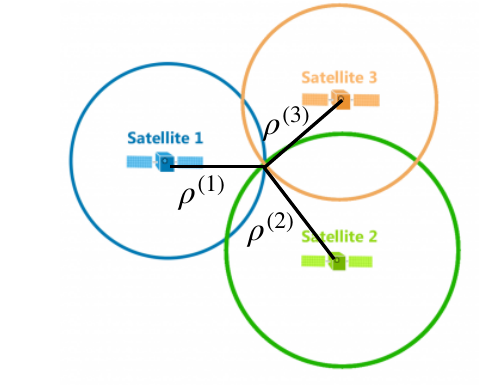
\includegraphics[scale=0.280]{img/hardware/gnss_1.jpeg}
\end{center}
\caption{Trilateration in 2D.}
\label{gnss_1}
\end{figure}


If we have exactly four satellites, we can solve for
the receiver position, $\mathbf{r}$, and the receiver clock error, $\Delta t_r$,  explicitly. If we have more than four, we can use the method of
least squares to find the maximum likelihood position
assuming Gaussian noise. GPS suffers from multiple error sources. First, charged ions in the ionosphere can delay
the signal by an unknown amount. Surrounding terrain and buildings
may cause reflections that increase the distance traveled by
the signal before reaching the receiver, these are called multi-path errors. Any small error in
clock synchronization or satellite position information can
have catastrophic consequences. Even a one microsecond
timing error can lead to a significant error in
position, 300 meters. Both a Ephemeris data
and satellite clocks are updated and recalibrated often, but the calibration can be out of date. Finally, the geometric configuration of visible satellites can also lead to
variations in positioning accuracy. This is known as the geometric
dilution of precision. For higher accuracy, a configuration with satellites spread across
the sky is preferable. 

Luckily, for some applications, we can improve GNSS accuracy by
augmenting the system in various ways. Differential GPS can correct receiver positioning
estimates by making use of the more accurately known positions
of one or more fixed base stations. Corrections are broadcast
on separate frequencies to the GNSS receiver in the moving vehicle. Real-Time Kinematic, or
RTK GPS makes use of carrier phase information to improve positioning accuracy down to
two centimeters in some cases. Although both of these techniques can significantly improve
the accuracy of GPS, they are typically quite
costly to implement. Inertial sensors are very
useful for navigation. However, they drift or accumulate
unbounded error over time. The GPS system in contrast, provides bounded error
positioning updates. A self-driving car equipped
with GPS will maintain a guaranteed level of positioning
accuracy at all times, unless the GPS receiver fails or loses
track of at least four satellites. 

\subsection{Summary}

To summarize, the Global Navigation Satellite
Systems work by combining pseudoranges from at least four
satellites to determine a 3D position. GPS or GNSS error can come from several different sources
including ionospheric delays, multi-path effects, and also possibly from the geometric
dilution of precision. In order to improve GNSS accuracy, techniques like differential GPS
or RTK GPS can be used.  We can fuse inertial
measurements from IMUs with position measurements
from a GPS to produce an accurate localization estimate
for a self-driving car. The sensors are complementary
and they're used together in practically all self-driving cars.

\subsection{Questions}

\subsection{Assignements}
 






\section{Sensor Noise and Aliasing}
\label{sensor_noise_aliasing}

The previous sections described various  types of sensors commonly used in robotics and autonomous vehicles in particular. However, the truth is that all sensors
are subject to noise and aliasing that is  the nonuniqueness of sensor readings. Let's briefly discuss these two
issues.

\subsection{Sensor Noise}
\label{sensor_noise}
As it is understandable, sensors provide are the fundamental input for the process of perception. Thus, the degree to which sensors can discriminate
the world state is essential. Sensor noise indices a limitation on the consistency of sensor readings in the same environmental
state and thus on the number of useful bits available from each sensor reading. Often, the source of sensor noise problems is that
some environmental features are not captured by the robot's representaion and hence overlloked \cite{Siegwart2011}.

\begin{framed}
\begin{exmp}

For example, a vision system used for indoor navigation in an office building may use
the color values detected by its color CCD camera. When the sun is hidden by clouds, the 
illusmination of the building's interior changes because of the windows throughtout the building. This results
in the hue values not being constant. The color CCD appears noisy from the robot's prespective as if subject
to random error. The hue values obtained from the CCD camera will be unusable unless the robot is able
to note the position of the sun and the clouds in its representation.
\end{exmp}
\end{framed}


\begin{framed}
\begin{remark}{\textbf{More Noise}}


Illumination dependence is only one example of the apparent noise in a vision-based
sensor system. Picture jitter, signal gain, blooming, and blurring are all additional sources
of noise, potentially reducing the useful content of a color video image.

\end{remark}
\end{framed}

\begin{framed}
\begin{exmp}

Consider the noise level (i.e., apparent random error) of ultrasonic range-measuring sensors (e.g., sonars). 
When a sonar transducer emits sound
toward a relatively smooth and angled surface, much of the signal will coherently reflect
away, failing to generate a return echo. Depending on the material characteristics, a small
amount of energy may return nonetheless. When this level is close to the gain threshold of
the sonar sensor, then the sonar will, at times, succeed and, at other times, fail to detect the
object. From the robot’s perspective, a virtually unchanged environmental state will result
in two different possible sonar readings: one short and one long. The poor signal-to-noise ratio of a sonar sensor 
is further confounded by interference between multiple sonar emitters \cite{Siegwart2011}. 
Often, research robots have between twelve and forty-eight sonars on a single platform. In acoustically reflective environments, multipath 
interference is possible between the sonar emissions of one transducer and the echo detection
circuitry of another transducer. The result can be dramatically large errors (i.e., underestimation) 
in ranging values due to a set of coincidental angles. Such errors occur rarely, less
than 1\% of the time, and are virtually random from the robot’s perspective.

\end{exmp}
\end{framed}

Hopefully, the two examples mentioned above, have convinced you that sensor noise reduces the useful information content of sensor readings.
The solution is to take multiple readings into account, employing temporal fusion
or multisensor fusion to increase the overall information content of the robot’s inputs.

\subsection{ Sensor Aliasing}
\label{sensor_aliasing}

A second shortcoming of mobile robot sensors causes them to yield little information content, 
further exacerbating the problem of perception and, thus, localization. 


\begin{framed}
\begin{remark}{\textbf{sensor aliasing}}

The problem, known as \textbf{sensor aliasing}, is a phenomenon that humans rarely encounter. 
The human sensory system, particularly the visual system, tends to receive unique inputs in each unique
local state. In other words, every different place looks different. The power of this unique
mapping is only apparent when one considers situations where this fails to hold. Consider
moving through an unfamiliar building that is completely dark. When the visual system
sees only black, one’s localization system quickly degrades. Another useful example is that
of a human-sized maze made from tall hedges. Such mazes have been created for centuries,
and humans find them extremely difficult to solve without landmarks or clues because,
without visual uniqueness, human localization competence degrades rapidly.

\end{remark}
\end{framed}

In robots, the nonuniqueness of sensor readings, or sensor aliasing, is the norm and not
the exception. 

\begin{framed}
\begin{exmp}

Consider a narrow-beam rangefinder such as an ultrasonic or infrared range-finder. 
This sensor provides range information in a single direction without any additional
data regarding material composition such as color, texture, and hardness. Even for a robot
with several such sensors in an array, there are a variety of environmental states that would
trigger the same sensor values across the array. Formally, there is a many-to-one mapping
from environmental states to the robot’s perceptual inputs. Thus, the robot’s percepts
cannot distinguish from among these many states. A classic problem with sonar-based
robots involves distinguishing between humans and inanimate objects in an indoor setting.
When facing an apparent obstacle in front of itself, should the robot say “Excuse me”
because the obstacle may be a moving human, or should the robot plan a path around the
object because it may be a cardboard box? With sonar alone, these states are aliased, and
differentiation is impossible.

\end{exmp}
\end{framed}

The problem posed to navigation because of sensor aliasing is that, even with noise-free
sensors, the amount of information is generally insufficient to identify the robot’s position
from a single-percept reading. Thus, techniques must be employed by the robot programmer that base the robot’s 
localization on a series of readings and, thus, sufficient information to recover the robot’s position over time.


\subsection{Effector Noise}
\label{effector_noise}

The challenges of localization do not lie with sensor technologies alone. Just as robot sensors are noisy, 
limiting the information content of the signal, so robot effectors are also
noisy. In particular, a single action taken by a mobile robot may have several different possible results, 
even though from the robot’s point of view the initial state before the action
was taken is well known \cite{Siegwart2011}.

In short, mobile robot effectors introduce uncertainty about future state. Therefore, the
simple act of moving tends to increase the uncertainty of a mobile robot. There are, of
course, exceptions. Using cognition, the motion can be carefully planned so as to minimize
this effect, and indeed sometimes to actually result in more certainty. Furthermore, when
the robot’s actions are taken in concert with careful interpretation of sensory feedback, it
can compensate for the uncertainty introduced by noisy actions using the information provided by the sensors.

First, however, it is important to understand the precise nature of the effector noise that
impacts mobile robots. It is important to note that, from the robot’s point of view, this error
in motion is viewed as an error in odometry, or the robot’s inability to estimate its own posi-
tion over time using knowledge of its kinematics and dynamics. The true source of error
generally lies in an incomplete model of the environment. For instance, the robot does not
model the fact that the floor may be sloped, the wheels may slip, and a human may push
the robot. All of these unmodeled sources of error result in inaccuracy between the physical
motion of the robot, the intended motion of the robot, and the proprioceptive sensor estimates of motion.


\section{Questions}


\begin{enumerate}
\item What do we mean with the term sensor noise? Why is it important to take it into account? 
\item What do we mean with the term sensor aliasing?
\item What is the problem posed to navigation due to sensor aliasing?
\end{enumerate}
 

\clearpage
\section{Answers to Questions}
\label{answer_questions}

{\textbf{Answer to questions in section \ref{introduction_self_driving_cars_questions}}}

\begin{enumerate}

\item Which of the following are components of longitudinal control? (Select all that apply)

\begin{itemize}
\item Braking and accelerating are components of longitudinal control. Thus, options 1 and 3 are correct
\end{itemize}

\item Which of the following is not an example of OEDR?

\begin{itemize}
\item Finding routes between locations is a long term planning problem and not OEDR. Hence, option 2 is correct.
\end{itemize}

\item Which of the following tasks would you expect a Level 2 system to perform? (Select all that apply)

\begin{itemize}
\item Options 1 and 3 are correct.
\end{itemize}

\item What is the distinction between Level 3 autonomy and Level 4 autonomy? 

\begin{itemize}
\item Option 4 is correct.  Level 3 systems cannot handle emergencies automatically and as a result require full user alertness.
\end{itemize}

\item What distinguishes Level 5 Autonomy from Level 4?

\begin{itemize}
\item Option 3 is correct. Level 5 systems can operate in any weather condition, on any road type or surface and in any scenario and remain safe.
\end{itemize}

\end{enumerate}

{\textbf{Answer to questions in section \ref{perception_questions}}}

\begin{enumerate}

\item Which of the following tasks are associated with perception? (Select all that apply) 
\begin{itemize}
\item Perception deals with position, motion estimation and object identification. Hence options 1 and 2 are correct.
\end{itemize}

\item Which of the following can be on road objects? (Select all that apply) 

\begin{itemize}
\item Potholes and vehicles are on road objects. So options 1 and 4 are correct.
\end{itemize}

\item Which of the following tasks pose challenges to perception? (Select all that apply) 

\begin{itemize}
\item All four choices pose challenges to perception
\end{itemize}

\item Which of the following sensors are used for ego localization? (Select all that apply) 


\begin{itemize}
\item Global Navigation Satellite System (GNSS) sensor provides position and velocity measurements, and can be used to estimate vehicle position and orientation for localization. An IMU provide acceleration and rotation rate measurements from accelerometers and gyroscopes, and can be used to estimate vehicle orientation and aid in localization in general. Thus, options 1 and four are correct.
\end{itemize}

\item Which of the following objects would be relevant for perception in adaptive cruise control?


\begin{itemize}
\item Adaptive cruise control detects vehicles ahead to control speed and to maintain safe driving distances. So
option 3 is correct. 
\end{itemize}

\end{enumerate}



\bibliographystyle{plain}
\input{references.bbl}
\end{document}
